% !TeX program = xelatex
% !TeX encoding = UTF-8

\documentclass[12pt,a4paper]{article}

% thêm svg vào, nhưng khó dùng, chưa sài
\usepackage[inkscapelatex=false]{svg}

% cho dòng đầu thụt vào
\usepackage{indentfirst} 

% vẽ khung cho trang bìa
\usepackage{tikz}
\usetikzlibrary{calc}

% Gói để xoay ngang trang PDF
\usepackage{pdflscape} 


% dùng để canh giữa ô cho table
\usepackage{tabularray}

%===========================================================
% PACKAGES FOR VIETNAMESE SUPPORT AND FORMATTING
%===========================================================
\usepackage{fontspec}
\usepackage{xunicode}
\usepackage{xltxtra}

% Vietnamese language support
\usepackage[vietnamese]{babel}

% Font setup for XeLaTeX
\setmainfont{Times New Roman}
\setsansfont{Arial}
\setmonofont{Courier New}

%===========================================================
% ADDITIONAL PACKAGES
%===========================================================
\usepackage{geometry}
\usepackage{float}  
\usepackage{graphicx}
\usepackage{array}
\usepackage{booktabs}
\usepackage{longtable}
\usepackage{multirow}
\usepackage{enumitem}
\usepackage{titlesec}
\usepackage{fancyhdr}
\usepackage{titling}
\usepackage{tocloft}
\usepackage{hyperref}
\usepackage{xcolor}
\usepackage{amsmath}
\usepackage{amssymb}
\usepackage{tikz}
\usetikzlibrary{shapes,arrows,positioning,fit,backgrounds,calc}

% For code listings (SQL, etc.)
\usepackage{listings}
\lstset{
    basicstyle=\ttfamily\small,
    breaklines=true,
    frame=single,
    backgroundcolor=\color{gray!10},
    keywordstyle=\color{blue},
    commentstyle=\color{green!60!black},
    stringstyle=\color{red},
    showstringspaces=false,
    tabsize=2,
    captionpos=b
}

%===========================================================
% PAGE GEOMETRY
%===========================================================
\geometry{
    left=2.5cm,
    right=2.5cm,
    top=2.5cm,
    bottom=2.5cm
}

%===========================================================
% HYPERREF SETUP
%===========================================================
\hypersetup{
    colorlinks=true,
    linkcolor=blue,
    filecolor=magenta,
    urlcolor=cyan,
    citecolor=green,
    pdftitle={Báo Cáo 1: Phân Rã - Hệ Thống Quản Lý Thư Viện},
    pdfauthor={Nhóm 2 - Lớp AI2005},
    pdfsubject={Database Systems - DBI202},
    pdfkeywords={library, database, ERD, decomposition}
}

%===========================================================
% TITLE FORMATTING
%===========================================================
\titleformat{\section}
  {\normalfont\LARGE\bfseries}{\thesection.}{0.5em}{\MakeUppercase}

\titleformat{\subsection}
  {\normalfont\Large\bfseries}{\thesubsection.}{0.5em}{}

\titleformat{\subsubsection}
  {\normalfont\large\bfseries}{\thesubsubsection.}{0.5em}{}

\titleformat{\paragraph}
  {\normalfont\normalsize\bfseries}{\theparagraph.}{0.5em}{}

\titlespacing*{\section}{0pt}{3.5ex plus 1ex minus .2ex}{2.3ex plus .2ex}
\titlespacing*{\subsection}{0pt}{3ex plus 1ex minus .2ex}{1.8ex plus .2ex}
\titlespacing*{\subsubsection}{0pt}{2.5ex plus 1ex minus .2ex}{1.5ex plus .2ex}
\titlespacing*{\paragraph}{0pt}{2ex plus .5ex minus .2ex}{1em}

% Định dạng số thứ tự rõ ràng
\renewcommand{\thesection}{\arabic{section}}
\renewcommand{\thesubsection}{\thesection.\arabic{subsection}}
\renewcommand{\thesubsubsection}{\thesubsection.\arabic{subsubsection}}

%===========================================================
% CUSTOM COMMANDS
%===========================================================
\newcommand{\titlename}[1]{\textbf{#1}}
\newcommand{\entity}[1]{\texttt{#1}}
\newcommand{\pk}[1]{\textbf{PK:} #1}
\newcommand{\fk}[1]{\textbf{FK:} #1}
\newcommand{\attr}[1]{\textit{#1}}

%===========================================================
% DOCUMENT BEGIN
%===========================================================
\begin{document}

%===========================================================
% TITLE PAGE WITH FRAME (KHUNG TRANG BÌA CHUẨN)
%===========================================================
\begin{titlepage}
    % --- BƯỚC 1: Ép lề trang này khớp với khung ---
    % Khung vẽ: Trái 3cm, Phải 2cm. 
    % Ta set lề văn bản: Trái 3.5cm, Phải 2.5cm (thụt vào 0.5cm so với khung để không dính nét vẽ)
    \newgeometry{left=3.5cm,right=2.5cm,top=2.5cm,bottom=2.5cm}

    \begin{tikzpicture}[overlay,remember picture]
        % Khung viền đậm bên ngoài
        \draw [line width=3pt]
            ($ (current page.north west) + (3.0cm,-2.0cm) $)
            rectangle
            ($ (current page.south east) + (-2.0cm,2.0cm) $);
        % Khung viền mảnh bên trong
        \draw [line width=1pt]
            ($ (current page.north west) + (3.15cm,-2.15cm) $)
            rectangle
            ($ (current page.south east) + (-2.15cm,2.15cm) $);
    \end{tikzpicture}

    \centering % Lệnh này sẽ canh giữa toàn bộ nội dung theo lề mới
    \vspace{0.5cm}
    
    % Tên trường
    {\large \textbf{ĐẠI HỌC FPT}}\\
    {\large \textbf{FPT UNIVERSITY}}
    
    \vspace{1.5cm}
    
    % Logo trường
    \includegraphics[width=4cm]{images/logo.png} 
    \vspace{1cm}

    % Tên bài báo cáo
    {\Large \textbf{BÁO CÁO MÔN HỌC}}\\
    \vspace{0.5cm}
    {\Huge \textbf{XÂY DỰNG HỆ THỐNG CSDL\\ QUẢN LÝ THƯ VIỆN}}
    \vspace{0.5cm}
    
    % Tên tiếng Anh
    {\large \textbf{(BUILDING A DATABASE SYSTEM FOR\\ LIBRARY MANAGEMENT)}}

    \vspace{1.5cm}

    % Thông tin môn học (Dùng bảng để thẳng hàng nhưng vẫn canh giữa trang)
    \begin{tabular}{r l} % r l : Cột trái canh phải, cột phải canh trái -> Tạo hiệu ứng đẹp ở giữa
        \textbf{MÔN HỌC:} & HỆ THỐNG CƠ SỞ DỮ LIỆU \\
        \textbf{MÃ MÔN:}  & DBI202 \\
        \textbf{LỚP:}     & SE2043 \\
    \end{tabular}

    \vspace{1.5cm}

    % --- BƯỚC 2: Canh giữa phần thông tin nhóm ---
    % Bỏ flushright, dùng centering trong minipage
    \begin{minipage}{0.8\textwidth} % Rộng 80% trang để dễ canh
        \centering
        \textbf{GIẢNG VIÊN HƯỚNG DẪN:}\\
        TS. VŨ THANH PHONG
        \vspace{0.5cm}
        
        \textbf{NHÓM THỰC HIỆN (NHÓM 3):}\\
        \vspace{0.2cm}
        % Bảng danh sách sinh viên
        \begin{tabular}{l l} 
        1. & Nguyễn Ngọc Phúc \\
        2. & Thân Nhật Huy \\
        3. & Võ Hoàng Đình Trường \\ 
        4. & Nguyễn Thành An \\
        5. & Nguyễn Quang Thiên Phú \\
        6. & Phạm Ngọc Hưng \\
        \end{tabular}
    \end{minipage}

    \vfill

    % Ngày tháng
    \textbf{TP. HỒ CHÍ MINH, THÁNG 01 NĂM 2026}
    \vspace{1cm}

    % --- BƯỚC 3: Trả lại lề chuẩn cho các trang sau ---
    \restoregeometry
\end{titlepage}

%===========================================================
% TABLE OF CONTENTS
%===========================================================
\tableofcontents
\newpage

%===========================================================
% SECTION 0: INTRODUCTION
%===========================================================
\section{GIỚI THIỆU TỔNG QUAN}

\subsection{Phân tích bối cảnh và vấn đề bài toán}

\subsubsection{Bối cảnh bài toán}

Một thư viện cần xây dựng một hệ thống cơ sở dữ liệu để lưu trữ và quản lý toàn bộ thông tin liên quan đến các hoạt động quản lý sách và dịch vụ cho độc giả. Hệ thống này phải đảm bảo khả năng theo dõi thông tin chi tiết về các cuốn sách (\entity{BOOK}), các tác giả (\entity{AUTHOR}), nhà xuất bản (\entity{PUBLISHER}), bản sao sách (\entity{BOOK\_COPY}), và thành viên thư viện (\entity{MEMBER}). Dữ liệu bao gồm thông tin xuất bản, thông tin mượn/trả sách, tình trạng sách, và các khoản phí phạt khi trả sách muộn.

\subsubsection{Vấn đề cần giải quyết}

Bài toán đặt ra là phải thiết kế một mô hình cơ sở dữ liệu quan hệ có khả năng biểu diễn chính xác các mối quan hệ phức tạp giữa các thực thể nói trên. Cụ thể:

\begin{itemize}
    \item Mỗi cuốn sách có thể có nhiều tác giả, và mỗi tác giả có thể viết nhiều sách (mối quan hệ nhiều-nhiều).
    \item Mỗi cuốn sách có thể có nhiều bản sao, và mỗi bản sao có thể được mượn bởi một thành viên tại một thời điểm.
    \item Mỗi cuốn sách được xuất bản bởi một nhà xuất bản duy nhất.
    \item Thành viên thư viện có thể mượn nhiều sách, và mỗi lần mượn cần lưu trữ thông tin ngày mượn, ngày hết hạn, ngày trả, và khoản phí phạt (nếu có).
    \item Hệ thống phải hỗ trợ các báo cáo: sách được mượn nhiều nhất, lịch sử mượn sách của thành viên, các sách quá hạn, và thống kê sách theo tác giả hoặc nhà xuất bản.
\end{itemize}

Do đó, yêu cầu cốt lõi của bài toán là phân tích, xác định các thực thể, thuộc tính, và mối quan hệ giữa chúng, sau đó chuẩn hóa dữ liệu để đảm bảo tính toàn vẹn, tránh dư thừa và hỗ trợ truy vấn hiệu quả cho hoạt động quản lý của thư viện.

\subsection{Yêu cầu chức năng từ người dùng}

Dựa trên nhu cầu quản lý thư viện, cơ sở dữ liệu phải hỗ trợ các chức năng sau:

\subsubsection{Quản lý sách (Book Management)}

\textbf{Yêu cầu:}
\begin{itemize}
    \item Lưu trữ thông tin chi tiết về các cuốn sách, bao gồm:
    \begin{itemize}
        \item Mã sách (\attr{BookID}) - định danh duy nhất
        \item Tên sách (\attr{Title})
        \item Thể loại/Sự phân loại (\attr{SubjectCategory})
        \item Năm xuất bản (\attr{PublicationYear})
        \item Nhà xuất bản (\attr{Publisher})
    \end{itemize}
\end{itemize}

\textbf{Mục đích:} Hệ thống có thể tra cứu, tìm kiếm và quản lý danh mục sách hiệu quả.

\subsubsection{Quản lý tác giả (Author Management)}

\textbf{Yêu cầu:}
\begin{itemize}
    \item Lưu trữ thông tin chi tiết về các tác giả:
    \begin{itemize}
        \item Mã tác giả (\attr{AuthorID}) - định danh duy nhất
        \item Tên tác giả (\attr{Name})
        \item Quốc tịch (\attr{Nationality})
        \item Năm sinh (\attr{YearOfBirth})
    \end{itemize}
\end{itemize}

\textbf{Mục đích:} Theo dõi danh mục tác giả và các tác phẩm của họ.

\subsubsection{Quản lý nhà xuất bản (Publisher Management)}

\textbf{Yêu cầu:}
\begin{itemize}
    \item Lưu trữ thông tin về các nhà xuất bản:
    \begin{itemize}
        \item Mã nhà xuất bản (\attr{PublisherID}) - định danh duy nhất
        \item Tên nhà xuất bản (\attr{Name})
        \item Địa chỉ (\attr{Address})
        \item Số điện thoại liên hệ (\attr{ContactNumber})
    \end{itemize}
\end{itemize}

\textbf{Mục đích:} Quản lý thông tin đối tác cung cấp sách.

\subsubsection{Quản lý bản sao sách (Book Copy Management)}

\textbf{Yêu cầu:}
\begin{itemize}
    \item Lưu trữ thông tin về từng bản sao vật lý của sách:
    \begin{itemize}
        \item Mã bản sao (\attr{CopyID}) - định danh duy nhất
        \item Tình trạng (\attr{Condition}) - mới, cũ, hư hại
        \item Trạng thái (\attr{Status}) - có sẵn, đang mượn, bảo dưỡng
    \end{itemize}
\end{itemize}

\textbf{Mục đích:} Theo dõi chính xác số lượng sách sẵn sàng cho mượn.

\subsubsection{Quản lý thành viên (Member Management)}

\textbf{Yêu cầu:}
\begin{itemize}
    \item Lưu trữ thông tin thành viên thư viện:
    \begin{itemize}
        \item Mã thành viên (\attr{MemberID}) - định danh duy nhất
        \item Tên thành viên (\attr{Name})
        \item Địa chỉ (\attr{Address})
        \item Số điện thoại (\attr{PhoneNumber})
        \item Loại thành viên (\attr{MembershipType}) - sinh viên, giảng viên, độc giả thường
    \end{itemize}
\end{itemize}

\textbf{Mục đích:} Quản lý thông tin độc giả và phân loại quyền lợi.

\subsubsection{Quản lý mượn/trả sách (Loan Management)}

\textbf{Yêu cầu:}
\begin{itemize}
    \item Lưu trữ chi tiết các giao dịch mượn/trả:
    \begin{itemize}
        \item Mã mượn (\attr{LoanID}) - định danh duy nhất
        \item Ngày mượn (\attr{BorrowDate})
        \item Ngày hết hạn (\attr{DueDate})
        \item Ngày trả (\attr{ReturnDate})
        \item Phí phạt quá hạn (\attr{OverdueFine}) - tính theo ngày
    \end{itemize}
\end{itemize}

\textbf{Mục đích:} Theo dõi luồng sách mượn/trả và tính toán phí phạt.

\subsubsection{Báo cáo thống kê (Reporting Requirements)}

\textbf{Yêu cầu:}
\begin{itemize}
    \item \textbf{Sách được mượn nhiều nhất:} Tổng hợp số lần mượn của từng sách
    \item \textbf{Lịch sử mượn của thành viên:} Xem tất cả sách một thành viên đã mượn
    \item \textbf{Sách quá hạn:} Liệt kê sách chưa trả và quá hạn
    \item \textbf{Thống kê theo tác giả:} Số lượng sách và lượt mượn theo từng tác giả
    \item \textbf{Thống kê theo nhà xuất bản:} Số lượng sách theo từng nhà xuất bản
\end{itemize}

\textbf{Mục đích:} Hỗ trợ quản lý ra quyết định về mua sách, điều chỉnh quy định, và cải thiện dịch vụ.

\subsection{Phạm vi dự án và công cụ sử dụng}

\subsubsection{Phạm vi dự án}

\textbf{Trong phạm vi dự án (In Scope):}
\begin{itemize}
    \item Phân tích yêu cầu và thiết kế sơ đồ ERD
    \item Chuyển đổi ERD sang mô hình quan hệ (Relational Data Model)
    \item Chuẩn hóa cơ sở dữ liệu đến 3NF (Third Normal Form)
    \item Định nghĩa lược đồ cơ sở dữ liệu với các ràng buộc (Constraints)
    \item Triển khai cơ sở dữ liệu trên SQL Server
    \item Thêm dữ liệu mẫu (Sample Data)
    \item Tạo các stored procedures, functions, và triggers
    \item Viết các câu lệnh SQL truy vấn cho báo cáo
\end{itemize}

\textbf{Ví dụ về các câu truy vấn SQL cần triển khai:}
\begin{itemize}
    \item Liệt kê tất cả các tác phẩm của một tác giả cụ thể
    \item Tìm các thành viên đang mượn sách quá hạn
    \item Thống kê sách được mượn nhiều nhất
    \item Tính tổng phí phạt của một thành viên
    \item Lấy lịch sử mượn sách của một thành viên
\end{itemize}

\textbf{Ngoài phạm vi dự án (Out of Scope):}
\begin{itemize}
    \item Giao diện người dùng đồ họa (GUI/Web Application)
    \item Hệ thống thanh toán điện tử
    \item Quản lý kho phức tạp (đặt hàng, nhập hàng)
    \item Hệ thống thông báo tự động (email/SMS)
    \item Phân tích dữ liệu nâng cao (Data Analytics)
    \item Quản lý người dùng và phân quyền chi tiết
\end{itemize}

\subsubsection{Công cụ sử dụng}

\begin{table}[H]
\centering
\caption{Công cụ và công nghệ sử dụng}
\begin{tabular}{@{}|l|l|l|@{}}
\hline
\textbf{Công cụ} & \textbf{Mục đích} & \textbf{Lý do chọn} \\ \hline
SQL Server & Hệ quản trị CSDL & Đáng tin cậy, hỗ trợ T-SQL đầy đủ \\ \hline
SSMS & Công cụ phát triển & Giao diện trực quan, hỗ trợ debug T-SQL \\ \hline
draw.io & Tạo sơ đồ ERD & Công cụ trực quan, hỗ trợ AI \\ \hline
T-SQL & Ngôn ngữ truy vấn & Ngôn ngữ chuẩn của SQL Server \\ \hline
Git/GitHub & Quản lý phiên bản & Theo dõi thay đổi mã nguồn \\ \hline
Word/Markdown & Tài liệu hóa & Tạo báo cáo và tài liệu kỹ thuật \\ \hline
\end{tabular}
\end{table}

%===========================================================
% SECTION 1: REPORT 1 - DECOMPOSITION
%===========================================================
\section{BÁO CÁO 1: PHÂN RÃ}

\subsection{Phân công nhiệm vụ}

\begin{table}[H]
\centering
\caption{Phân công nhiệm vụ nhóm}
\begin{tabular}{@{}|c|l|p{8cm}|c|@{}}
\hline
\textbf{STT} & \textbf{Họ và tên} & \textbf{Phân công nhiệm vụ} & \textbf{Điểm} \\ \hline
1 & Nguyễn Ngọc Phúc &
Phân tích yêu cầu hệ thống, tham gia thiết kế ERD, xây dựng các thực thể và mối quan hệ, tổng hợp nội dung báo cáo &
10 \\ \hline
2 & Thân Nhật Huy &
Phân tích yêu cầu hệ thống, tham gia thiết kế ERD, xây dựng các thực thể và mối quan hệ, hỗ trợ viết báo cáo &
10 \\ \hline
3 & Võ Hoàng Đình Trường &
Phân tích yêu cầu hệ thống, tham gia thiết kế ERD, xác định thuộc tính và ràng buộc dữ liệu, hỗ trợ kiểm tra tài liệu &
10 \\ \hline
4 & Nguyễn Thành An &
Phân tích yêu cầu hệ thống, tham gia thiết kế ERD, xác định mối quan hệ giữa các thực thể, hỗ trợ hoàn thiện báo cáo &
10 \\ \hline
5 & Nguyễn Quang Thiên Phú &
Phân tích yêu cầu hệ thống, tham gia thiết kế ERD, chuẩn hóa mô hình dữ liệu, rà soát nội dung báo cáo &
10 \\ \hline
6 & Phạm Ngọc Hưng &
Phân tích yêu cầu hệ thống, tham gia thiết kế ERD, kiểm tra tính nhất quán của mô hình, tổng hợp và chỉnh sửa báo cáo &
10 \\ \hline
\end{tabular}
\end{table}


\subsection{Cơ sở lý thuyết}

\subsubsection{Khái niệm về Phân rã (Decomposition)}

Phân rã trong thiết kế cơ sở dữ liệu là quá trình đầu tiên và quan trọng nhất trong việc chuyển đổi các yêu cầu nghiệp vụ phức tạp thành một mô hình dữ liệu có cấu trúc. Quá trình này bao gồm:

\textbf{1. Xác định Thực thể (Entity Identification):}
\begin{itemize}
    \item Nhận diện các đối tượng chính trong hệ thống cần quản lý
    \item Mỗi thực thể đại diện cho một danh mục (category) của dữ liệu
    \item Ví dụ: \entity{BOOK} (Sách), \entity{MEMBER} (Thành viên), \entity{LOAN} (Mượn/trả)
\end{itemize}

\textbf{2. Xác định Thuộc tính (Attribute Identification):}
\begin{itemize}
    \item Mô tả các đặc điểm chi tiết của từng thực thể
    \item Phân loại thuộc tính: đơn (simple), phức hợp (composite), đa trị (multi-valued), dẫn xuất (derived)
    \item Xác định khóa chính (Primary Key) để định danh duy nhất
\end{itemize}

\textbf{3. Xác định Mối quan hệ (Relationship Identification):}
\begin{itemize}
    \item Mô tả sự liên kết giữa các thực thể
    \item Xác định bội số (cardinality): 1-1, 1-N, N-M
    \item Xác định tính chất (optionality): bắt buộc hoặc tùy chọn
\end{itemize}

\textbf{Kết quả:} Sơ đồ Thực thể - Mối quan hệ (Entity-Relationship Diagram - ERD), giúp trực quan hóa cấu trúc dữ liệu trước khi chuyển đổi sang mô hình quan hệ.

\subsubsection{Các thành phần chính trong mô hình E/R}

\textbf{1. Entity (Thực thể):}
\begin{itemize}
    \item \textbf{Định nghĩa:} Là tập hợp các đối tượng có cùng đặc điểm và thuộc tính
    \item \textbf{Biểu diễn:} Hình chữ nhật trong ERD
    \item \textbf{Đặc điểm:} Có tên duy nhất, có khóa chính (Primary Key) để định danh
\end{itemize}

\textbf{2. Attribute (Thuộc tính):}
\begin{itemize}
    \item \textbf{Định nghĩa:} Mô tả các đặc trưng của thực thể hoặc mối quan hệ
    \item \textbf{Biểu diễn:} Hình ellip trong ERD
    \item \textbf{Phân loại:}
\end{itemize}

\begin{table}[H]
\centering
\caption{Phân loại thuộc tính}
\begin{tabular}{@{}|l|p{8cm}|l|@{}}
\hline
\textbf{Loại} & \textbf{Mô tả} & \textbf{Ví dụ} \\ \hline
Simple (Đơn) & Không thể chia nhỏ & Title, Year \\ \hline
Composite (Phức hợp) & Có thể chia nhỏ & Address = Street + City \\ \hline
Multi-valued (Đa trị) & Có nhiều giá trị & Phone numbers \\ \hline
Derived (Dẫn xuất) & Giá trị tính từ thuộc tính khác & Age = Year - BirthYear \\ \hline
Key (Khóa) & Định danh duy nhất & BookID, ISBN \\ \hline
\end{tabular}
\end{table}

\textbf{3. Relationship (Mối quan hệ):}
\begin{itemize}
    \item \textbf{Định nghĩa:} Mô tả sự liên kết giữa hai hoặc nhiều thực thể
    \item \textbf{Biểu diễn:} Hình thoi (diamond) trong ERD
    \item \textbf{Bội số (Cardinality):}
\end{itemize}

\begin{table}[H]
\centering
\caption{Các loại bội số}
\begin{tabular}{@{}|l|l|@{}}
\hline
\textbf{Loại} & \textbf{Ý nghĩa} \\ \hline
One-to-One (1:1) & Một bản ghi của A liên kết với một bản ghi của B \\ \hline
One-to-Many (1:N) & Một bản ghi của A liên kết với nhiều bản ghi của B \\ \hline
Many-to-Many (N:M) & Nhiều bản ghi của A liên kết với nhiều bản ghi của B \\ \hline
\end{tabular}
\end{table}

\subsubsection{Quy trình xác định E/R Diagram}

\textbf{Bước 1:} Phân tích yêu cầu bài toán - Đọc và hiểu rõ yêu cầu nghiệp vụ

\textbf{Bước 2:} Xác định các thực thể chính - Tìm các danh từ chính trong yêu cầu

\textbf{Bước 3:} Xác định mối quan hệ - Tìm các động từ mô tả sự liên kết

\textbf{Bước 4:} Liệt kê thuộc tính - Tìm các tính từ mô tả đặc điểm

\textbf{Bước 5:} Vẽ sơ đồ E/R - Sử dụng công cụ: draw.io, Visual Paradigm

\textbf{Bước 6:} Kiểm tra và hoàn thiện - Rà soát lại các yêu cầu

\subsection{Tập thực thể}

Sau khi phân tích yêu cầu bài toán, chúng tôi xác định được \textbf{6 thực thể chính} cần quản lý trong hệ thống thư viện:

\subsubsection{BOOK (SÁCH)}

\textbf{Mô tả thực thể:} Lưu trữ thông tin về các cuốn sách trong thư viện

\begin{table}[H]
\centering
\caption{Thuộc tính thực thể BOOK}
\begin{tabular}{@{}|l|l|p{6cm}|l|@{}}
\hline
\textbf{Thuộc tính} & \textbf{Kiểu dữ liệu} & \textbf{Mô tả} & \textbf{Ràng buộc} \\ \hline
\attr{BookID} & INT & Mã định danh duy nhất & PK, NOT NULL \\ \hline
\attr{ISBN} & VARCHAR(17) & Mã số tiêu chuẩn quốc tế & UNIQUE \\ \hline
\attr{Title} & VARCHAR(255) & Tên tiêu đề của sách & NOT NULL \\ \hline
\attr{SubjectCategory} & VARCHAR(100) & Thể loại phân loại sách & NULL \\ \hline
\attr{PublicationYear} & INT & Năm xuất bản sách & NULL \\ \hline
\attr{PublisherID} & INT & Mã nhà xuất bản & FK \\ \hline
\end{tabular}
\end{table}

\subsubsection{AUTHOR (TÁC GIẢ)}

\textbf{Mô tả thực thể:} Lưu trữ thông tin cá nhân về các tác giả của sách

\begin{table}[H]
\centering
\caption{Thuộc tính thực thể AUTHOR}
\begin{tabular}{@{}|l|l|p{6cm}|l|@{}}
\hline
\textbf{Thuộc tính} & \textbf{Kiểu dữ liệu} & \textbf{Mô tả} & \textbf{Ràng buộc} \\ \hline
\attr{AuthorID} & INT & Mã định danh duy nhất & PK, NOT NULL \\ \hline
\attr{Name} & VARCHAR(255) & Tên đầy đủ của tác giả & NOT NULL \\ \hline
\attr{Nationality} & VARCHAR(100) & Quốc tịch của tác giả & NULL \\ \hline
\attr{YearOfBirth} & INT & Năm sinh của tác giả & NULL \\ \hline
\end{tabular}
\end{table}

\subsubsection{PUBLISHER (NHÀ XUẤT BẢN)}

\textbf{Mô tả thực thể:} Lưu trữ thông tin về các nhà xuất bản

\begin{table}[H]
\centering
\caption{Thuộc tính thực thể PUBLISHER}
\begin{tabular}{@{}|l|l|p{6cm}|l|@{}}
\hline
\textbf{Thuộc tính} & \textbf{Kiểu dữ liệu} & \textbf{Mô tả} & \textbf{Ràng buộc} \\ \hline
\attr{PublisherID} & INT & Mã định danh duy nhất & PK, NOT NULL \\ \hline
\attr{Name} & VARCHAR(255) & Tên nhà xuất bản & NOT NULL \\ \hline
\attr{Address} & VARCHAR(500) & Địa chỉ của nhà xuất bản & NULL \\ \hline
\attr{ContactNumber} & VARCHAR(50) & Số điện thoại liên hệ & NULL \\ \hline
\end{tabular}
\end{table}

\subsubsection{BOOK\_COPY (BẢN SAO SÁCH)}

\textbf{Mô tả thực thể:} Lưu trữ thông tin về từng bản sao vật lý của sách

\begin{table}[H]
\centering
\caption{Thuộc tính thực thể BOOK\_COPY}
\begin{tabular}{@{}|l|l|p{6cm}|l|@{}}
\hline
\textbf{Thuộc tính} & \textbf{Kiểu dữ liệu} & \textbf{Mô tả} & \textbf{Ràng buộc} \\ \hline
\attr{CopyID} & INT & Mã định danh duy nhất của bản sao & PK, NOT NULL \\ \hline
\attr{BookID} & INT & Mã sách mà bản sao thuộc về & FK, NOT NULL \\ \hline
\attr{Condition} & VARCHAR(50) & Tình trạng bản sao & NULL \\ \hline
\attr{Status} & VARCHAR(20) & Trạng thái hiện tại & NOT NULL \\ \hline
\end{tabular}
\end{table}

\textbf{Ghi chú:}
\begin{itemize}
    \item \attr{Condition}: New (Mới), Good (Tốt), Fair (Trung bình), Poor (Kém)
    \item \attr{Status}: Available (Sẵn sàng), Borrowed (Đang mượn), Maintenance (Bảo dưỡng), Lost (Mất)
\end{itemize}

\subsubsection{MEMBER (THÀNH VIÊN)}

\textbf{Mô tả thực thể:} Lưu trữ thông tin về thành viên thư viện

\begin{table}[H]
\centering
\caption{Thuộc tính thực thể MEMBER}
\begin{tabular}{@{}|l|l|p{6cm}|l|@{}}
\hline
\textbf{Thuộc tính} & \textbf{Kiểu dữ liệu} & \textbf{Mô tả} & \textbf{Ràng buộc} \\ \hline
\attr{MemberID} & INT & Mã định danh duy nhất & PK, NOT NULL \\ \hline
\attr{Name} & VARCHAR(255) & Tên đầy đủ của thành viên & NOT NULL \\ \hline
\attr{Address} & VARCHAR(500) & Địa chỉ liên lạc & NULL \\ \hline
\attr{Phone} & VARCHAR(20) & Số điện thoại liên hệ & NULL \\ \hline
\attr{MembershipType} & VARCHAR(50) & Loại thành viên & NOT NULL \\ \hline
\end{tabular}
\end{table}

\textbf{Ghi thích:} \attr{MembershipType}: Student (Sinh viên), Faculty (Giảng viên), Standard (Thông thường), Premium (VIP)

\subsubsection{LOAN (MƯỢN/TRẢ)}

\textbf{Mô tả thực thể:} Lưu trữ thông tin về các giao dịch mượn/trả sách

\begin{table}[H]
\centering
\caption{Thuộc tính thực thể LOAN}
\begin{tabular}{@{}|l|l|p{6cm}|l|@{}}
\hline
\textbf{Thuộc tính} & \textbf{Kiểu dữ liệu} & \textbf{Mô tả} & \textbf{Ràng buộc} \\ \hline
\attr{LoanID} & INT & Mã định danh duy nhất & PK, NOT NULL \\ \hline
\attr{MemberID} & INT & Mã thành viên mượn & FK, NOT NULL \\ \hline
\attr{CopyID} & INT & Mã bản sao được mượn & FK, NOT NULL \\ \hline
\attr{BorrowDate} & DATE & Ngày mượn sách & NOT NULL \\ \hline
\attr{DueDate} & DATE & Ngày hết hạn phải trả & NOT NULL \\ \hline
\attr{ReturnDate} & DATE & Ngày thực tế trả sách & NULL \\ \hline
\attr{OverdueFine} & DECIMAL(10,2) & Phí phạt quá hạn & DEFAULT 0 \\ \hline
\end{tabular}
\end{table}

\subsubsection{Tổng hợp thực thể}

\begin{table}[H]
\centering
\caption{Bảng tổng hợp 6 thực thể chính}
\begin{tabular}{|c|l|l|l|}
\hline
\textbf{\#} & \textbf{Tên thực thể} & \textbf{Mô tả} & \textbf{Khóa chính} \\ \hline
1 & \entity{BOOK} & Danh mục sách trong thư viện & \attr{BookID} \\ \hline
2 & \entity{AUTHOR} & Danh mục tác giả & \attr{AuthorID} \\ \hline
3 & \entity{PUBLISHER} & Danh mục nhà xuất bản & \attr{PublisherID} \\ \hline
4 & \entity{BOOK\_COPY} & Các bản sao vật lý của sách & \attr{CopyID} \\ \hline
5 & \entity{MEMBER} & Thành viên thư viện & \attr{MemberID} \\ \hline
6 & \entity{LOAN} & Giao dịch mượn/trả sách & \attr{LoanID} \\ \hline
\end{tabular}
\end{table}

\subsection{Các mối quan hệ}

Sau khi xác định các thực thể, chúng tôi phân tích và xác định được \textbf{5 mối quan hệ chính}:

\begin{table}[H]
\centering
\caption{Bảng tổng hợp 5 mối quan hệ}
\begin{tabular}{|c|l|l|l|c|p{5cm}|}
\hline
\textbf{\#} & \textbf{Tên} & \textbf{Thực thể 1} & \textbf{Thực thể 2} & \textbf{Bội số} & \textbf{Mô tả} \\ \hline
1 & Publishes & \entity{PUBLISHER} & \entity{BOOK} & 1 : N & Một nhà XB xuất bản nhiều sách \\ \hline
2 & Writes & \entity{AUTHOR} & \entity{BOOK} & M : N & Tác giả viết sách (qua BOOK\_AUTHOR) \\ \hline
3 & Has & \entity{BOOK} & \entity{BOOK\_COPY} & 1 : N & Một sách có nhiều bản sao vật lý \\ \hline
4 & Processes & \entity{MEMBER} & \entity{LOAN} & 1 : N & Thành viên tạo nhiều giao dịch mượn \\ \hline
5 & Records & \entity{LOAN} & \entity{BOOK\_COPY} & 1 : 1 & Một giao dịch ghi nhận một bản sao \\ \hline
\end{tabular}
\end{table}


\textbf{Ghi thích về cấu trúc mối quan hệ:}

\begin{itemize}
    \item \textbf{Quan hệ mượn sách:} Thành viên không trực tiếp kết nối đến bản sao sách. Thay vào đó, một thành viên tạo một giao dịch \entity{LOAN}, và giao dịch đó ghi nhận bản sao sách cụ thể được mượn.
    \item Cấu trúc này cho phép lưu trữ đầy đủ thông tin về mỗi lần mượn: ngày mượn, ngày hết hạn, ngày trả, và phí phạt.
    \item Điều này cũng cho phép theo dõi lịch sử mượn của một thành viên qua thời gian.
\end{itemize}

\subsection{Thuộc tính chi tiết}

\subsubsection{Bảng trung gian BOOK\_AUTHOR}

Vì mối quan hệ giữa \entity{AUTHOR} và \entity{BOOK} là nhiều-nhiều (M:N), chúng tôi cần một bảng trung gian:

\begin{table}[H]
\centering
\caption{Bảng trung gian BOOK\_AUTHOR}
\begin{tabular}{@{}|l|l|p{6cm}|l|@{}}
\hline
\textbf{Thuộc tính} & \textbf{Kiểu dữ liệu} & \textbf{Mô tả} & \textbf{Ràng buộc} \\ \hline
\attr{BookID} & INT & Khóa ngoại tham chiếu BOOK & PK, FK \\ \hline
\attr{AuthorID} & INT & Khóa ngoại tham chiếu AUTHOR & PK, FK \\ \hline
\end{tabular}
\end{table}

\textbf{Ràng buộc:} PRIMARY KEY (\attr{BookID}, \attr{AuthorID}) - Khóa chính kép

% \begin{landscape} % Bắt đầu xoay ngang trang này
\subsection{Sơ đồ Thực thể - Mối quan hệ (ERD)}

\subsubsection{Sơ đồ ERD hoàn chỉnh}
% https://dbdiagram.io/d/dbi-697adba5bd82f5fce2f72136
\begin{figure}[H]
\centering
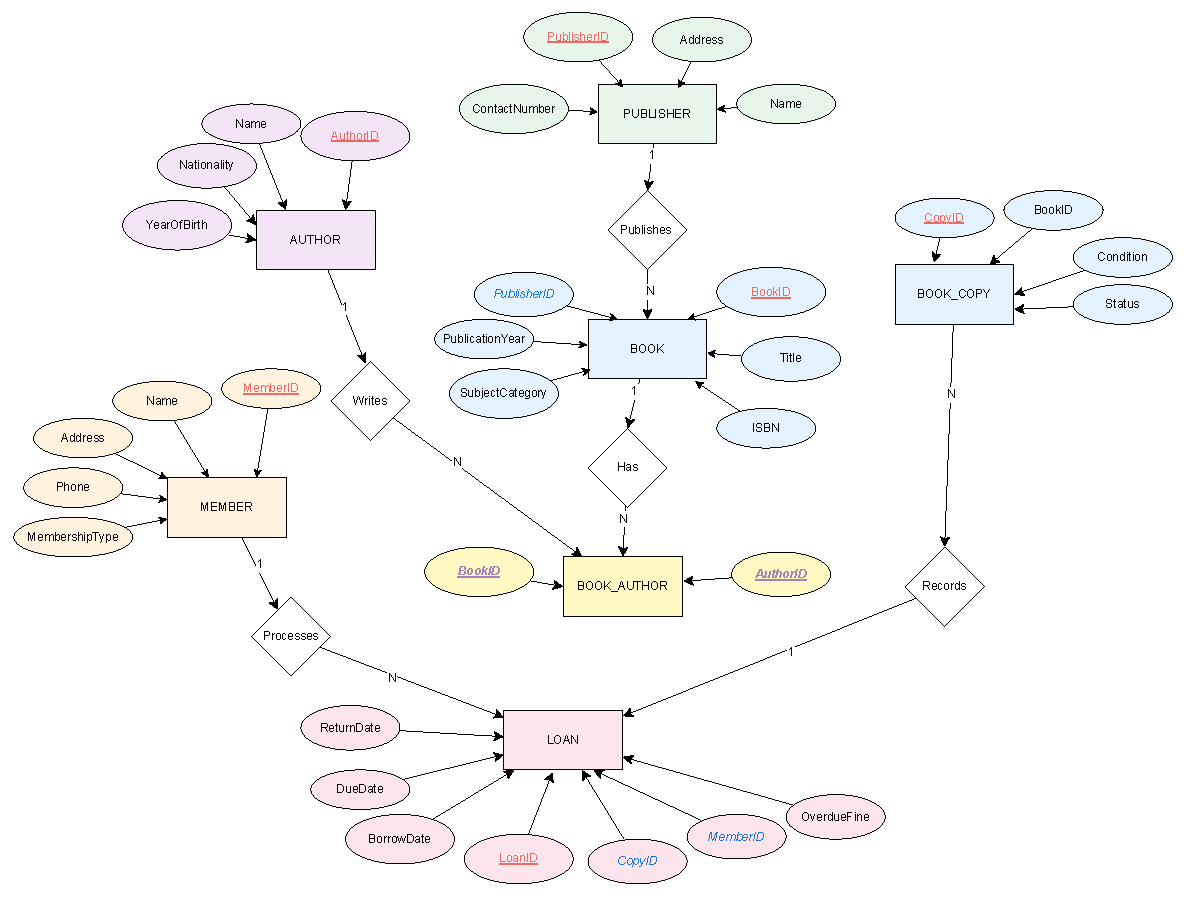
\includegraphics[width=\textwidth]{images/Library_Management_ERD_hinhthoi.drawio.pdf}
\caption{Sơ đồ Thực thể - Mối quan hệ (ERD) cho hệ thống Quản lý Thư viện}
\label{fig:erd}
\end{figure}
% \end{landscape} % Kết thúc xoay ngang, trang sau sẽ tự về dọc lại

\textbf{Chú thích ký hiệu trong sơ đồ:}
\begin{itemize}
\item Khóa chính (Primary Key - PK): Được viết bằng chữ màu đỏ và gạch chân (Ví dụ: BookID, AuthorID, LoanID).
\item Khóa ngoại (Foreign Key - FK): Được viết bằng chữ màu xanh dương và in nghiêng (Ví dụ: PublisherID trong bảng BOOK, MemberID trong bảng LOAN).
\item Khóa chính vừa là Khóa ngoại (PK, FK): -Được viết bằng chữ màu tím, vừa gạch chân vừa in nghiêng.
\end{itemize}


\subsubsection{Mô tả chi tiết các mối quan hệ}

\textbf{1. Publishes (1:N) - PUBLISHER đến BOOK}
\begin{itemize}
    \item Một nhà xuất bản có thể xuất bản nhiều cuốn sách
    \item Mỗi cuốn sách được xuất bản bởi đúng một nhà xuất bản
    \item Ràng buộc: \attr{PublisherID} trong \entity{BOOK} là khóa ngoại tham chiếu đến \entity{PUBLISHER}
\end{itemize}

\textbf{2. Writes (M:N) - AUTHOR đến BOOK}
\begin{itemize}
    \item Một tác giả có thể viết nhiều cuốn sách
    \item Một cuốn sách có thể có nhiều tác giả
    \item Cần bảng trung gian \entity{BOOK\_AUTHOR} để quản lý mối quan hệ này
    \item Bảng \entity{BOOK\_AUTHOR} có khóa chính kép (\attr{BookID}, \attr{AuthorID})
\end{itemize}

\textbf{3. Has (1:N) - BOOK đến BOOK\_COPY}
\begin{itemize}
    \item Một cuốn sách (title) có thể có nhiều bản sao vật lý
    \item Mỗi bản sao thuộc về một cuốn sách duy nhất
    \item Ràng buộc: \attr{BookID} trong \entity{BOOK\_COPY} là khóa ngoại tham chiếu đến \entity{BOOK}
    \item Khi xóa sách, tất cả bản sao cũng bị xóa (ON DELETE CASCADE)
\end{itemize}

\textbf{4. Processes (1:N) - MEMBER đến LOAN}
\begin{itemize}
    \item Một thành viên có thể tạo nhiều giao dịch mượn
    \item Mỗi giao dịch mượn thuộc về một thành viên
    \item Ràng buộc: \attr{MemberID} trong \entity{LOAN} là khóa ngoại tham chiếu đến \entity{MEMBER}
    \item Lưu trữ lịch sử đầy đủ của các giao dịch mượn/trả
\end{itemize}

\textbf{5. Records (1:1) - LOAN đến BOOK\_COPY}
\begin{itemize}
    \item Một giao dịch mượn ghi nhận một bản sao sách cụ thể
    \item Mỗi bản sao tại một thời điểm chỉ được ghi nhận trong một giao dịch đang hoạt động
    \item Ràng buộc: \attr{CopyID} trong \entity{LOAN} là khóa ngoại tham chiếu đến \entity{BOOK\_COPY}
    \item Không thể có hai giao dịch mượn đang hoạt động cho cùng một bản sao
\end{itemize}

\textbf{Lưu ý về thiết kế:}
\begin{itemize}
    \item Thành viên không trực tiếp kết nối đến bản sao sách
    \item Việc mượn sách được thực hiện thông qua thực thể \entity{LOAN}
    \item Thiết kế này cho phép lưu trữ đầy đủ thông tin về mỗi lần mượn: ngày mượn, ngày hết hạn, ngày trả, và phí phạt
    \item Hỗ trợ truy vấn lịch sử mượn của thành viên và thống kê báo cáo
\end{itemize}

\subsubsection{Các quyết định thiết kế chính}

\textbf{1. Tách BOOK và BOOK\_COPY:}
\begin{itemize}
    \item \entity{BOOK} lưu thông tin chung về title/ISBN
    \item \entity{BOOK\_COPY} lưu thông tin về từng bản sao vật lý
    \item Giúp quản lý chính xác số lượng sách có sẵn
\end{itemize}

\textbf{2. Sử dụng bảng trung gian BOOK\_AUTHOR:}
\begin{itemize}
    \item Hỗ trợ mối quan hệ M:N giữa \entity{AUTHOR} và \entity{BOOK}
    \item Cho phép một sách có nhiều tác giả
    \item Cho phép một tác giả có nhiều sách
\end{itemize}

\textbf{3. Tách LOAN thành thực thể riêng:}
\begin{itemize}
    \item Lưu trữ đầy đủ thông tin về mỗi giao dịch mượn
    \item Hỗ trợ tính toán phí phạt
    \item Lưu trữ lịch sử mượn/trả đầy đủ
\end{itemize}

\subsection{Kết luận báo cáo 1}

\subsubsection{Tổng kết kết quả}

Báo cáo 1 đã hoàn thành phân tích và thiết kế sơ đồ ERD cho hệ thống quản lý thư viện:

\textbf{1. Xác định được 6 thực thể chính:}
\begin{itemize}
    \item \entity{BOOK} - 6 thuộc tính
    \item \entity{AUTHOR} - 4 thuộc tính
    \item \entity{PUBLISHER} - 4 thuộc tính
    \item \entity{BOOK\_COPY} - 4 thuộc tính
    \item \entity{MEMBER} - 5 thuộc tính
    \item \entity{LOAN} - 7 thuộc tính
\end{itemize}

\textbf{2. Xác định được 5 mối quan hệ:}
\begin{itemize}
    \item Publishes (1:N) - \entity{PUBLISHER} → \entity{BOOK}
    \item Writes (M:N) - \entity{AUTHOR} ↔ \entity{BOOK} (qua \entity{BOOK\_AUTHOR})
    \item Has (1:N) - \entity{BOOK} → \entity{BOOK\_COPY}
    \item Processes (1:N) - \entity{MEMBER} → \entity{LOAN}
    \item Records (1:1) - \entity{LOAN} → \entity{BOOK\_COPY}
\end{itemize}

\textbf{Lưu ý về thiết kế quan hệ:}
\begin{itemize}
    \item Việc mượn sách được mô hình hóa thông qua thực thể \entity{LOAN}, không phải quan hệ trực tiếp giữa \entity{MEMBER} và \entity{BOOK\_COPY}
    \item Thành viên tạo giao dịch \entity{LOAN}, và giao dịch đó ghi nhận bản sao sách được mượn
    \item Thiết kế này cho phép lưu trữ đầy đủ thông tin về mỗi lần mượn và theo dõi lịch sử
\end{itemize}

\textbf{3. Xác định được 1 bảng trung gian:}
\begin{itemize}
    \item \entity{BOOK\_AUTHOR} - quản lý mối quan hệ nhiều-nhiều
\end{itemize}


%===========================================================
% SECTION 2: REPORT 2 - RELATIONAL MODEL DESIGN
%===========================================================
\newpage
\section{BÁO CÁO 2: MÔ HÌNH QUAN HỆ (RELATIONAL DATA MODEL)}

\subsection{Giới thiệu báo cáo 2}

Báo cáo 2 là bước tiếp theo trong quá trình thiết kế cơ sở dữ liệu, chuyển đổi từ sơ đồ Thực thể - Mối quan hệ (ERD) đã hoàn thiện trong Báo cáo 1 sang \textbf{Mô hình Quan hệ (Relational Data Model)}. Đây là bước quan trọng để chuẩn bị cho quá trình chuẩn hóa dữ liệu trong Báo cáo 3.

\textbf{Mục tiêu của Báo cáo 2:}
\begin{itemize}
    \item Chuyển đổi các thực thể (entities) thành các bảng (tables/relation schemas)
    \item Xác định khóa chính (Primary Keys) và khóa ngoại (Foreign Keys)
    \item Thiết lập các mối quan hệ giữa các bảng thông qua khóa ngoại
    \item Xác định các phụ thuộc hàm (Functional Dependencies)
    \item Nhận dạng các mẫu chưa chuẩn hóa để chuẩn bị cho chuẩn hóa 3NF
\end{itemize}

\subsection{Cơ sở lý thuyết}

\subsubsection{Mô hình Quan hệ (Relational Model)}

\textbf{Định nghĩa:} Mô hình quan hệ là một mô hình cơ sở dữ liệu thể hiện dữ liệu dưới dạng các quan hệ (relations), mà người dùng có thể nhận thức dưới dạng các bảng (tables) gồm các hàng (rows) và cột (columns).

\textbf{Các thành phần cơ bản:}

\begin{table}[H]
\centering
\caption{Thành phần của Mô hình Quan hệ}
\begin{tabular}{@{}|l|p{9cm}|@{}}
\hline
\textbf{Thành phần} & \textbf{Mô tả} \\ \hline
\textbf{Relation (Quan hệ)} & Một bảng 2D chứa dữ liệu, tương ứng với một thực thể trong ERD \\ \hline
\textbf{Tuple (Bộ)} & Một hàng trong bảng, tương ứng với một bản ghi hoặc một thể hiện của thực thể \\ \hline
\textbf{Attribute (Thuộc tính)} & Một cột trong bảng, tương ứng với một thuộc tính của thực thể \\ \hline
\textbf{Domain (Miền giá trị)} & Tập hợp các giá trị hợp lệ cho một thuộc tính \\ \hline
\textbf{Degree (Bậc)} & Số lượng thuộc tính trong một quan hệ \\ \hline
\textbf{Cardinality (Độ)} & Số lượng bộ trong một quan hệ \\ \hline
\end{tabular}
\end{table}

\subsubsection{Khóa chính (Primary Key)}

\textbf{Định nghĩa:} Khóa chính là một thuộc tính hoặc tập hợp các thuộc tính định danh duy nhất mỗi bộ trong một quan hệ.

\textbf{Đặc điểm:}
\begin{itemize}
    \item \textbf{Tính duy nhất:} Không có hai bộ nào có cùng giá trị khóa chính
    \item \textbf{Tính không rỗng:} Khóa chính không thể chứa giá trị NULL
    \item \textbf{Tính ổn định:} Giá trị khóa chính không nên thay đổi
\end{itemize}

\textbf{Ký hiệu:} Gạch dưới thuộc tính (ví dụ: \underline{BookID}) hoặc ký hiệu PK

\subsubsection{Khóa ngoại (Foreign Key)}

\textbf{Định nghĩa:} Khóa ngoại là một thuộc tính trong một quan hệ tham chiếu đến khóa chính của một quan hệ khác, thiết lập mối quan hệ giữa hai bảng.

\textbf{Đặc điểm:}
\begin{itemize}
    \item \textbf{Tham chiếu:} Giá trị khóa ngoại phải khớp với giá trị khóa chính được tham chiếu, hoặc là NULL
    \item \textbf{Tính toàn vẹn:} Đảm bảo tính toàn vẹn tham chiếu (Referential Integrity)
    \item \textbf{Hành vi cascade:} Xác định điều gì xảy ra khi dữ liệu được tham chiếu bị xóa hoặc cập nhật
\end{itemize}

\textbf{Ký hiệu:} Chỉ mũi tên từ khóa ngoại sang khóa chính được tham chiếu

\subsubsection{Phụ thuộc hàm (Functional Dependency)}

\textbf{Định nghĩa:} Phụ thuộc hàm là một ràng buộc giữa hai tập hợp thuộc tính trong một quan hệ. Được ký hiệu là $X \rightarrow Y$, đọc là "X xác định Y" hoặc "Y phụ thuộc hàm vào X".

\textbf{Định nghĩa toán học:} Trong một quan hệ R, $X \rightarrow Y$ nếu và chỉ nếu mỗi giá trị của X liên kết với chính xác một giá trị của Y.

\textbf{Ví dụ:}
\begin{itemize}
    \item \texttt{BookID} $\rightarrow$ \texttt{Title}: Mã sách xác định tên sách
    \item \texttt{BookID} $\rightarrow$ \texttt{ISBN, PublicationYear, PublisherID}
    \item \texttt{MemberID} $\rightarrow$ \texttt{Name, Address, Phone}
\end{itemize}

\subsection{Quy tắc chuyển đổi từ ERD sang Mô hình Quan hệ}

\subsubsection{Quy tắc cơ bản}

\begin{table}[H]
\centering
\caption{Quy tắc chuyển đổi ERD sang Relational Model}
\begin{tabular}{@{}|l|p{9cm}|@{}}
\hline
\textbf{Thành phần ERD} & \textbf{Quy tắc chuyển đổi} \\ \hline
\textbf{Thực thể mạnh} & Chuyển thành một bảng (table) riêng biệt \\ \hline
\textbf{Thuộc tính} & Chuyển thành cột (column) của bảng \\ \hline
\textbf{Khóa chính} & Chuyển thành PRIMARY KEY constraint \\ \hline
\textbf{Quan hệ 1:1} & Thêm khóa ngoại vào một trong hai bảng, thường là bảng có tham gia bắt buộc \\ \hline
\textbf{Quan hệ 1:N} & Thêm khóa ngoại vào bảng "N" (bên nhiều) tham chiếu đến bảng "1" (bên một) \\ \hline
\textbf{Quan hệ M:N} & Tạo bảng trung gian (junction table) với hai khóa ngoại \\ \hline
\textbf{Thực thể yếu} & Thêm khóa ngoại tham chiếu đến thực thể sở hữu, có thể tạo khóa chính kép \\ \hline
\end{tabular}
\end{table}

\subsubsection{Quy tắc chi tiết cho từng loại quan hệ}

\textbf{1. Quan hệ Một-Nhiều (1:N):}

\begin{itemize}
    \item Bên "1": Thực thể có khóa chính PK
    \item Bên "N": Thêm thuộc tính khóa ngoại FK tham chiếu đến PK của bên "1"
    \item \textbf{Ví dụ:} \entity{PUBLISHER} (1) $\rightarrow$ \entity{BOOK} (N)
    \item \entity{BOOK} có \attr{PublisherID} là khóa ngoại tham chiếu đến \entity{PUBLISHER}
\end{itemize}

\textbf{2. Quan hệ Nhiều-Nhiều (M:N):}

\begin{itemize}
    \item Tạo bảng trung gian mới
    \item Bảng trung gian có hai khóa ngoại FK tham chiếu đến PK của hai thực thể
    \item Khóa chính của bảng trung gian là kết hợp của hai khóa ngoại
    \item \textbf{Ví dụ:} \entity{AUTHOR} (M) $\leftrightarrow$ \entity{BOOK} (N)
    \item Tạo \entity{BOOK\_AUTHOR} với PK (\attr{BookID}, \attr{AuthorID})
\end{itemize}

\textbf{3. Quan hệ Một-Một (1:1):}

\begin{itemize}
    \item Thêm khóa ngoại vào một trong hai bảng
    \item Khóa ngoại vừa là khóa ngoại vừa là khóa chính
    \item \textbf{Ví dụ:} \entity{LOAN} (1) $\leftrightarrow$ \entity{BOOK\_COPY} (1)
    \item \entity{LOAN} có \attr{CopyID} là FK và tham chiếu độc nhất
\end{itemize}

\subsection{Chuyển đổi ERD sang Lược đồ Quan hệ}

\subsubsection{Lược đồ quan hệ cho các thực thể cơ bản}

\textbf{1. PUBLISHER (Nhà xuất bản)}

$$
\texttt{PUBLISHER}(\underline{\texttt{PublisherID}}, \texttt{Name}, \texttt{Address}, \texttt{ContactNumber})
$$

\begin{table}[H]
\centering
\caption{Lược đồ quan hệ PUBLISHER}
\begin{tabular}{@{}|l|l|l|l|@{}}
\hline
\textbf{Tên bảng} & \textbf{Khóa chính} & \textbf{Thuộc tính} & \textbf{Kiểu dữ liệu} \\ \hline
\multirow{4}{*}{\texttt{PUBLISHER}} & \multirow{4}{*}{\underline{\texttt{PublisherID}}} & \texttt{PublisherID} & INT \\ \cline{3-4}
& & \texttt{Name} & VARCHAR(255) \\ \cline{3-4}
& & \texttt{Address} & VARCHAR(500) \\ \cline{3-4}
& & \texttt{ContactNumber} & VARCHAR(50) \\ \hline
\end{tabular}
\end{table}

\textbf{2. AUTHOR (Tác giả)}

$$
\texttt{AUTHOR}(\underline{\texttt{AuthorID}}, \texttt{Name}, \texttt{Nationality}, \texttt{YearOfBirth})
$$

\begin{table}[H]
\centering
\caption{Lược đồ quan hệ AUTHOR}
\begin{tabular}{@{}|l|l|l|l|@{}}
\hline
\textbf{Tên bảng} & \textbf{Khóa chính} & \textbf{Thuộc tính} & \textbf{Kiểu dữ liệu} \\ \hline
\multirow{4}{*}{\texttt{AUTHOR}} & \multirow{4}{*}{\underline{\texttt{AuthorID}}} & \texttt{AuthorID} & INT \\ \cline{3-4}
& & \texttt{Name} & VARCHAR(255) \\ \cline{3-4}
& & \texttt{Nationality} & VARCHAR(100) \\ \cline{3-4}
& & \texttt{YearOfBirth} & INT \\ \hline
\end{tabular}
\end{table}

\textbf{3. MEMBER (Thành viên)}

$$
\texttt{MEMBER}(\underline{\texttt{MemberID}}, \texttt{Name}, \texttt{Address}, \texttt{Phone}, \texttt{MembershipType})
$$

\begin{table}[H]
\centering
\caption{Lược đồ quan hệ MEMBER}
\begin{tabular}{@{}|l|l|l|l|@{}}
\hline
\textbf{Tên bảng} & \textbf{Khóa chính} & \textbf{Thuộc tính} & \textbf{Kiểu dữ liệu} \\ \hline
\multirow{5}{*}{\texttt{MEMBER}} & \multirow{5}{*}{\underline{\texttt{MemberID}}} & \texttt{MemberID} & INT \\ \cline{3-4}
& & \texttt{Name} & VARCHAR(255) \\ \cline{3-4}
& & \texttt{Address} & VARCHAR(500) \\ \cline{3-4}
& & \texttt{Phone} & VARCHAR(20) \\ \cline{3-4}
& & \texttt{MembershipType} & VARCHAR(50) \\ \hline
\end{tabular}
\end{table}

\textbf{4. BOOK (Sách)}

$$
\texttt{BOOK}(\underline{\texttt{BookID}}, \texttt{ISBN}, \texttt{Title}, \texttt{SubjectCategory}, \texttt{PublicationYear}, \texttt{PublisherID})
$$

\begin{table}[H]
\centering
\caption{Lược đồ quan hệ BOOK}
\begin{tblr}{
  colspec = {|c|c|c|l|l|}, % Định dạng cột: Giữa | Giữa | Giữa | Trái | Trái
  vlines, hlines,          % Kẻ khung
  rows = {m},              % Căn giữa dọc tất cả các hàng
  row{1} = {font=\bfseries, c}, % Dòng tiêu đề: In đậm, căn giữa
  cell{2}{1} = {r=6}{c},   % Ô BOOK: Gộp 6 hàng, căn giữa
  cell{2}{2} = {r=6}{c},   % Ô BookID: Gộp 6 hàng, căn giữa
  cell{2}{3} = {r=6}{c},        % Ô PublisherID: Gộp 6 hàng, căn giữa
}
Tên bảng & Khóa chính & Khóa ngoại & Thuộc tính & Kiểu dữ liệu \\
BOOK     & \underline{BookID} & PublisherID & BookID           & INT \\
         &            &            & ISBN             & VARCHAR(17) \\
         &            &            & Title            & VARCHAR(255) \\
         &            &            & SubjectCategory  & VARCHAR(100) \\
         &            &            & PublicationYear  & INT \\
         &            &            & PublisherID      & INT \\
\end{tblr}
\end{table}

\textbf{Ghi chú:}
\begin{itemize}
    \item \texttt{PublisherID} là khóa ngoại tham chiếu đến \texttt{PUBLISHER(PublisherID)}
    \item Ký hiệu: $\texttt{BOOK.PublisherID} \rightarrow \texttt{PUBLISHER.PublisherID}$
\end{itemize}

\textbf{5. BOOK\_COPY (Bản sao sách)}

$$
\texttt{BOOK\_COPY}(\underline{\texttt{CopyID}}, \texttt{BookID}, \texttt{Condition}, \texttt{Status})
$$

\begin{table}[H]
\centering
\caption{Lược đồ quan hệ BOOK\_COPY}
\begin{tblr}{
  colspec = {|c|c|c|l|l|}, 
  vlines, hlines,
  rows = {m},
  row{1} = {font=\bfseries, c},
  cell{2}{1} = {r=4}{c}, % Gộp 4 hàng cho tên bảng
  cell{2}{2} = {r=4}{c}, % Gộp 4 hàng cho khóa chính
  cell{2}{3} = {r=4}{c}, % Gộp 4 hàng cho khóa ngoại
}
Tên bảng & Khóa chính & Khóa ngoại & Thuộc tính & Kiểu dữ liệu \\
BOOK\_COPY & \underline{CopyID} & BookID & CopyID & INT \\
           &           &        & BookID & INT \\
           &           &        & Condition & VARCHAR(50) \\
           &           &        & Status    & VARCHAR(20) \\
\end{tblr}
\end{table}

\textbf{Ghi chú:}
\begin{itemize}
    \item \texttt{BookID} là khóa ngoại tham chiếu đến \texttt{BOOK(BookID)}
    \item Đây là thực thể yếu (weak entity) phụ thuộc vào \texttt{BOOK}
    \item Ký hiệu: $\texttt{BOOK\_COPY.BookID} \rightarrow \texttt{BOOK.BookID}$
\end{itemize}

\textbf{6. LOAN (Mượn/trả)}

$$
\texttt{LOAN}(\underline{\texttt{LoanID}}, \texttt{MemberID}, \texttt{CopyID}, \texttt{BorrowDate}, \texttt{DueDate}, \texttt{ReturnDate}, \texttt{OverdueFine})
$$

\begin{table}[H]
\centering
\caption{Lược đồ quan hệ LOAN}
\begin{tblr}{
  colspec = {|c|c|c|l|l|}, % 5 cột: Giữa, Giữa, Giữa, Trái, Trái
  vlines, hlines,
  rows = {m},            % Căn giữa dọc cho tất cả các ô
  row{1} = {font=\bfseries, c}, % Dòng đầu in đậm và căn giữa ngang
  cell{2}{1} = {r=7}{c}, % Gộp 7 hàng cho tên bảng LOAN
  cell{2}{2} = {r=7}{c}, % Gộp 7 hàng cho khóa chính LoanID
  cell{2}{3} = {r=7}{c}, % Gộp 7 hàng cho các khóa ngoại
}
Tên bảng & Khóa chính & Khóa ngoại & Thuộc tính & Kiểu dữ liệu \\
LOAN     & \underline{LoanID} & {MemberID, \\ CopyID} & LoanID & INT \\
         &            &            & MemberID     & INT \\
         &            &            & CopyID       & INT \\
         &            &            & BorrowDate   & DATE \\
         &            &            & DueDate      & DATE \\
         &            &            & ReturnDate   & DATE \\
         &            &            & OverdueFine  & DECIMAL(10,2) \\
\end{tblr}
\end{table}

\textbf{Ghi chú:}
\begin{itemize}
    \item \texttt{MemberID} là khóa ngoại tham chiếu đến \texttt{MEMBER(MemberID)}
    \item \texttt{CopyID} là khóa ngoại tham chiếu đến \texttt{BOOK\_COPY(CopyID)}
    \item Ký hiệu:
    \begin{itemize}
        \item $\texttt{LOAN.MemberID} \rightarrow \texttt{MEMBER.MemberID}$
        \item $\texttt{LOAN.CopyID} \rightarrow \texttt{BOOK\_COPY.CopyID}$
    \end{itemize}
\end{itemize}

\subsubsection{Bảng trung gian cho quan hệ M:N}

\textbf{BOOK\_AUTHOR (Bảng trung gian Sách-Tác giả)}

$$
\texttt{BOOK\_AUTHOR}(\underline{\texttt{BookID}}, \underline{\texttt{AuthorID}})
$$

\begin{table}[H]
\centering
\caption{Lược đồ quan hệ BOOK\_AUTHOR (Bảng trung gian)}
\begin{tblr}{
  colspec = {|c|c|X[l]|X[l]|}, % Cột X sẽ tự động co giãn để vừa khít trang giấy
  vlines, hlines,
  rows = {m},                 % Căn giữa dọc
  row{1} = {font=\bfseries, c}, % Dòng tiêu đề in đậm, căn giữa ngang
  cell{2}{1} = {r=2}{c},      % Gộp 2 hàng cho tên bảng
  cell{2}{2} = {r=2}{c},      % Gộp 2 hàng cho khóa chính kép
}
Tên bảng & Khóa chính & Khóa ngoại & Mô tả \\
BOOK\_AUTHOR & \underline{BookID}, \underline{AuthorID} & BookID $\rightarrow$ BOOK (BookID) & Khóa ngoại đến BOOK \\
             &                                          & AuthorID $\rightarrow$ AUTHOR (AuthorID) & Khóa ngoại đến AUTHOR \\
\end{tblr}
\end{table}

\textbf{Ghi chú:}
\begin{itemize}
    \item \textbf{Khóa chính kép:} (\texttt{BookID}, \texttt{AuthorID})
    \item Mỗi cặp (BookID, AuthorID) là duy nhất - một tác giả chỉ được liệt kê một lần cho mỗi sách
    \item Quan hệ này thể hiện mối quan hệ nhiều-nhiều giữa \texttt{AUTHOR} và \texttt{BOOK}
\end{itemize}

\subsection{Tổng hợp Lược đồ Quan hệ Hệ Thống}

\subsubsection{Tất cả Lược đồ Quan hệ}

\textbf{Tóm tắt tất cả 7 bảng trong hệ thống:}

\begin{table}[H]
\centering
\renewcommand{\arraystretch}{1.5} % Giúp các dòng giãn cách thoáng hơn
\begin{tabular}{l p{12cm}}
\textbf{PUBLISHER} & (\underline{PublisherID}, Name, Address, ContactNumber) \\
\textbf{AUTHOR}    & (\underline{AuthorID}, Name, Nationality, YearOfBirth) \\
\textbf{MEMBER}    & (\underline{MemberID}, Name, Address, Phone, MembershipType) \\
\textbf{BOOK}      & (\underline{BookID}, ISBN, Title, SubjectCategory, PublicationYear, PublisherID$^*$) \\
\textbf{BOOK\_COPY} & (\underline{CopyID}, BookID$^\dagger$, Condition, Status) \\
\textbf{LOAN}      & (\underline{LoanID}, MemberID$^\ddagger$, CopyID$^\ddagger$, BorrowDate, DueDate, ReturnDate, OverdueFine) \\
\textbf{BOOK\_AUTHOR} & (\underline{BookID}$^\dagger$, \underline{AuthorID}$^\ddagger$) \\
\end{tabular}
\end{table}

\vspace{0.3cm}
\noindent \textbf{Chú thích:}
\begin{itemize}[leftmargin=1.5cm, labelsep=0.3cm, itemsep=0pt]
    \item[$^*, \dagger, \ddagger$] Các ký hiệu phía sau tên thuộc tính chỉ \textbf{Khóa ngoại} (Foreign Key) tham chiếu đến bảng tương ứng.
    \item[\underline{\hspace{0.3cm}}] Các thuộc tính được gạch chân đóng vai trò là \textbf{Khóa chính} (Primary Key).
\end{itemize}

\begin{table}[H]
\centering
\caption{Tổng hợp các bảng và khóa}
\begin{tblr}{
  colspec = {|c|l|l|X[l]|}, % Cột cuối tự động giãn rộng
  vlines, hlines,
  rows = {m},                 % Căn giữa dọc cho tất cả các hàng
  row{1} = {font=\bfseries, c}, % Dòng tiêu đề: In đậm, căn giữa ngang
  cell{7}{1,2,3} = {r=2}{l},    % Gộp hàng cho bảng LOAN
  cell{9}{1,2,3} = {r=2}{l},    % Gộp hàng cho bảng BOOK_AUTHOR
}
STT & Tên bảng & Khóa chính (PK) & Khóa ngoại (FK) \\
1 & PUBLISHER   & PublisherID & -- \\
2 & AUTHOR      & AuthorID    & -- \\
3 & MEMBER      & MemberID    & -- \\
4 & BOOK        & BookID      & PublisherID $\rightarrow$ PUBLISHER \\
5 & BOOK\_COPY  & CopyID      & BookID $\rightarrow$ BOOK \\
6 & LOAN        & LoanID      & MemberID $\rightarrow$ MEMBER \\
  &             &             & CopyID $\rightarrow$ BOOK\_COPY \\
7 & BOOK\_AUTHOR & BookID, AuthorID & BookID $\rightarrow$ BOOK \\
  &             &                   & AuthorID $\rightarrow$ AUTHOR \\
\end{tblr}
\end{table}

\subsubsection{Sơ đồ Mô hình Quan hệ (Relational Data Model Diagram)}

% TODO: Insert your RDM diagram here
% Replace the filename below with your actual diagram file
\begin{figure}[H]
\centering
\includegraphics[width=\textwidth,keepaspectratio]{images/RDM_Library_Management.pdf}
% \includegraphics[width=\textwidth,keepaspectratio]{images/RDM_Library_Management.png}
\caption{Sơ đồ Mô hình Quan hệ (Relational Data Model) cho hệ thống Quản lý Thư viện}
\label{fig:rdm}
\end{figure}

\textbf{Ghi chú ký hiệu trong sơ đồ:}
\begin{itemize}
\item \textbf{PK (Primary Key):} Khóa chính - được hiển thị ở đầu danh sách cột, có gạch chân
\item \textbf{FK (Foreign Key):} Khóa ngoại - tham chiếu đến bảng khác
\item \textbf{Đường nối:} Thể hiện mối quan hệ giữa các bảng
\end{itemize}

\subsection{Phụ thuộc Hàm (Functional Dependencies)}

\subsubsection{Định nghĩa và Ký hiệu}

\textbf{Phụ thuộc hàm (Functional Dependency - FD)} mô tả mối quan hệ giữa các thuộc tính trong một bảng. Nếu thuộc tính X xác định thuộc tính Y, ta ký hiệu: $X \rightarrow Y$

\textbf{Ví dụ:} Nếu biết mã sách ($\texttt{BookID}$), ta biết được tên sách ($\texttt{Title}$), ISBN, năm xuất bản, và mã nhà xuất bản. Ký hiệu:
$$ \texttt{BookID} \rightarrow \texttt{Title, ISBN, PublicationYear, PublisherID} $$

\subsubsection{Các Phụ thuộc Hàm cho từng Bảng}

\textbf{1. Bảng PUBLISHER:}

$$
\begin{aligned}
\texttt{PublisherID} &\rightarrow \texttt{Name} \\
\texttt{PublisherID} &\rightarrow \texttt{Address} \\
\texttt{PublisherID} &\rightarrow \texttt{ContactNumber}
\end{aligned}
$$

\textbf{Gộp:} $\texttt{PublisherID} \rightarrow \texttt{Name, Address, ContactNumber}$

\textbf{Giải thích:} Mã nhà xuất bản xác định duy nhất tên, địa chỉ và số điện thoại liên hệ của nhà xuất bản đó.

\vspace{0.5cm}

\textbf{2. Bảng AUTHOR:}

$$
\begin{aligned}
\texttt{AuthorID} &\rightarrow \texttt{Name} \\
\texttt{AuthorID} &\rightarrow \texttt{Nationality} \\
\texttt{AuthorID} &\rightarrow \texttt{YearOfBirth}
\end{aligned}
$$

\textbf{Gộp:} $\texttt{AuthorID} \rightarrow \texttt{Name, Nationality, YearOfBirth}$

\textbf{Giải thích:} Mã tác giả xác định duy nhất tên, quốc tịch và năm sinh của tác giả đó.

\vspace{0.5cm}

\textbf{3. Bảng MEMBER:}

$$
\begin{aligned}
\texttt{MemberID} &\rightarrow \texttt{Name} \\
\texttt{MemberID} &\rightarrow \texttt{Address} \\
\texttt{MemberID} &\rightarrow \texttt{Phone} \\
\texttt{MemberID} &\rightarrow \texttt{MembershipType}
\end{aligned}
$$

\textbf{Gộp:} $\texttt{MemberID} \rightarrow \texttt{Name, Address, Phone, MembershipType}$

\textbf{Giải thích:} Mã thành viên xác định duy nhất tên, địa chỉ, số điện thoại và loại thành viên.

\vspace{0.5cm}

\textbf{4. Bảng BOOK:}

$$
\begin{aligned}
\texttt{BookID} &\rightarrow \texttt{ISBN} \\
\texttt{BookID} &\rightarrow \texttt{Title} \\
\texttt{BookID} &\rightarrow \texttt{SubjectCategory} \\
\texttt{BookID} &\rightarrow \texttt{PublicationYear} \\
\texttt{BookID} &\rightarrow \texttt{PublisherID}
\end{aligned}
$$


\begin{tblr}{
  colspec = {l X[l]}, % Cột 1: nhãn, Cột 2: nội dung tự xuống dòng
  colsep = 4pt,       % Khoảng cách giữa chữ "Gộp" và nội dung
}
\textbf{Gộp:} & $\texttt{BookID} \rightarrow \texttt{ISBN}, \texttt{Title}, \texttt{SubjectCategory}, \texttt{PublicationYear}, \texttt{PublisherID}$ \\
\end{tblr}


\textbf{Giải thích:} Mã sách xác định duy nhất ISBN, tên, thể loại, năm xuất bản và mã nhà xuất bản của sách đó.

\vspace{0.5cm}

\textbf{5. Bảng BOOK\_COPY:}

$$
\begin{aligned}
\texttt{CopyID} &\rightarrow \texttt{BookID} \\
\texttt{CopyID} &\rightarrow \texttt{Condition} \\
\texttt{CopyID} &\rightarrow \texttt{Status}
\end{aligned}
$$

\textbf{Gộp:} $\texttt{CopyID} \rightarrow \texttt{BookID, Condition, Status}$

\textbf{Giải thích:} Mã bản sao xác định duy nhất mã sách mà bản sao thuộc về, tình trạng và trạng thái hiện tại của bản sao.

\vspace{0.5cm}

\textbf{6. Bảng LOAN:}

$$
\begin{aligned}
\texttt{LoanID} &\rightarrow \texttt{MemberID} \\
\texttt{LoanID} &\rightarrow \texttt{CopyID} \\
\texttt{LoanID} &\rightarrow \texttt{BorrowDate} \\
\texttt{LoanID} &\rightarrow \texttt{DueDate} \\
\texttt{LoanID} &\rightarrow \texttt{ReturnDate} \\
\texttt{LoanID} &\rightarrow \texttt{OverdueFine}
\end{aligned}
$$


\begin{tblr}{
  colspec = {l X[l]},
  colsep = 4pt,
}
\textbf{Gộp:} & $\texttt{LoanID} \rightarrow \texttt{MemberID}, \texttt{CopyID}, \texttt{BorrowDate}, \texttt{DueDate}, \texttt{ReturnDate}, \texttt{OverdueFine}$ \\
\end{tblr}

\textbf{Giải thích:} Mã giao dịch mượn xác định duy nhất thành viên mượn, bản sao được mượn, ngày mượn, ngày hết hạn, ngày trả và phí phạt.

\vspace{0.5cm}

\textbf{7. Bảng BOOK\_AUTHOR (Bảng trung gian):}

Bảng này có khóa chính kép ($\texttt{BookID}, \texttt{AuthorID}$), nên không có phụ thuộc hàm từ một thuộc tính đơn lẻ. Các phụ thuộc hàm được xác định bởi cả hai khóa chính:

$$
\begin{aligned}
\texttt{BookID, AuthorID} &\rightarrow \texttt{BookID} \\
\texttt{BookID, AuthorID} &\rightarrow \texttt{AuthorID}
\end{aligned}
$$

\textbf{Giải thích:} Cả hai thuộc tính đều là một phần của khóa chính, không có phụ thuộc hàm từ khóa này sang khóa kia.

\subsubsection{Tổng hợp các Phụ thuộc Hàm}

\begin{table}[H]
\centering
\caption{Tổng hợp Phụ thuộc Hàm cho tất cả các bảng}
\begin{tblr}{
  colspec = {|l|X[l]|}, % Cột 1 tự vừa nội dung, Cột 2 tự giãn và xuống dòng
  vlines, hlines,
  rows = {m},            % Căn giữa dọc
  row{1} = {font=\bfseries, c}, % Tiêu đề in đậm, căn giữa
}
Bảng & Phụ thuộc Hàm \\
PUBLISHER & \texttt{PublisherID} $\rightarrow$ \texttt{Name}, \texttt{Address}, \texttt{ContactNumber} \\
AUTHOR    & \texttt{AuthorID} $\rightarrow$ \texttt{Name}, \texttt{Nationality}, \texttt{YearOfBirth} \\
MEMBER    & \texttt{MemberID} $\rightarrow$ \texttt{Name}, \texttt{Address}, \texttt{Phone}, \texttt{MembershipType} \\
BOOK      & \texttt{BookID} $\rightarrow$ \texttt{ISBN}, \texttt{Title}, \texttt{SubjectCategory}, \texttt{PublicationYear}, \texttt{PublisherID} \\
BOOK\_COPY & \texttt{CopyID} $\rightarrow$ \texttt{BookID}, \texttt{Condition}, \texttt{Status} \\
LOAN      & \texttt{LoanID} $\rightarrow$ \texttt{MemberID}, \texttt{CopyID}, \texttt{BorrowDate}, \texttt{DueDate}, \texttt{ReturnDate}, \texttt{OverdueFine} \\
BOOK\_AUTHOR & (\texttt{BookID}, \texttt{AuthorID}) $\rightarrow$ \texttt{BookID}, \texttt{AuthorID} (khóa chính kép) \\
\end{tblr}
\end{table}

\subsection{Đánh giá Mô hình Quan hệ}

\subsubsection{Tính toàn vẹn dữ liệu (Data Integrity)}

\textbf{1. Toàn vẹn thực thể (Entity Integrity):}
\begin{itemize}
    \item Mỗi bảng có khóa chính (Primary Key) xác định duy nhất mỗi dòng
    \item Khóa chính không chứa giá trị NULL
    \item Đảm bảo không có các bản ghi trùng lặp
\end{itemize}

\textbf{2. Toàn vẹn tham chiếu (Referential Integrity):}
\begin{itemize}
    \item Mọi khóa ngoại đều tham chiếu đến khóa chính hợp lệ của bảng khác
    \item Không thể có giá trị khóa ngoại "mồ côi" (orphaned records)
    \item Được thực thi thông qua ràng buộc FOREIGN KEY
\end{itemize}

\textbf{3. Toàn vẹn miền (Domain Integrity):}
\begin{itemize}
    \item Mỗi thuộc tính có kiểu dữ liệu phù hợp
    \item Giá trị thuộc tính nằm trong miền giá trị cho phép
    \item Các ràng buộc CHECK đảm bảo giá trị hợp lệ
\end{itemize}

\subsubsection{Ưu điểm của Mô hình Quan hệ hiện tại}

\begin{table}[H]
\centering
\caption{Ưu điểm thiết kế}
\begin{tabular}{@{}|l|p{10cm}|@{}}
\hline
\textbf{Thiết kế} & \textbf{Ưu điểm} \\ \hline
Tách BOOK và BOOK\_COPY & Quản lý chính xác số lượng bản sao vật lý của mỗi sách \\ \hline
Bảng trung gian BOOK\_AUTHOR & Hỗ trợ mối quan hệ M:N giữa tác giả và sách \\ \hline
Thực thể LOAN riêng biệt & Lưu trữ đầy đủ thông tin về mỗi giao dịch mượn \\ \hline
Khóa ngoại với CASCADE & Tự động đồng bộ dữ liệu khi xóa/cập nhật \\ \hline
\end{tabular}
\end{table}

\subsubsection{Hạn chế và Cải tiến tiềm năng}

\textbf{Các vấn đề cần chuẩn hóa trong Báo cáo 3:}

\begin{enumerate}
    \item \textbf{Phân tích 1NF (First Normal Form):}
    \begin{itemize}
        \item Kiểm tra xem tất cả thuộc tính có chứa giá trị nguyên thủy (atomic)
        \item Không có thuộc tính đa trị (multi-valued)
        \item Không có các nhóm lặp lại (repeating groups)
    \end{itemize}

    \item \textbf{Phân tích 2NF (Second Normal Form):}
    \begin{itemize}
        \item Kiểm tra các bảng có khóa chính kép (như \texttt{BOOK\_AUTHOR})
        \item Xác định phụ thuộc hàm một phần (partial dependencies)
        \item Loại bỏ các thuộc tính phụ thuộc vào một phần của khóa chính
    \end{itemize}

    \item \textbf{Phân tích 3NF (Third Normal Form):}
    \begin{itemize}
        \item Kiểm tra các phụ thuộc hàm truyền tải (transitive dependencies)
        \item Xác định các thuộc tính phi khóa phụ thuộc vào các thuộc tính phi khóa khác
        \item Tách các bảng để loại bỏ phụ thuộc truyền tải
    \end{itemize}
\end{enumerate}

\subsection{Nhận dạng các Bất thường (Anomaly Recognition)}

\subsubsection{Mục đích của việc nhận dạng bất thường}

Sau khi xác định các Phụ thuộc Hàm (Functional Dependencies) cho tất cả các bảng, bước tiếp theo là nhận dạng các bất thường tiềm ẩn trong cơ sở dữ liệu. Đây là preparation quan trọng cho quá trình chuẩn hóa (normalization) trong Báo cáo 3.

\subsubsection{Phân tích sơ bộ các bất thường}

\textbf{1. Bảng với khóa chính đơn (Single Primary Key):}

Các bảng \texttt{PUBLISHER}, \texttt{AUTHOR}, \texttt{MEMBER}, \texttt{BOOK}, \texttt{BOOK\_COPY}, và \texttt{LOAN} đều có khóa chính đơn. Dựa trên các FD đã xác định:

\begin{itemize}
    \item \textbf{Không có phụ thuộc hàm một phần (partial dependency)}: Vì tất cả các bảng đều có khóa chính đơn, không có thuộc tính nào phụ thuộc vào một phần của khóa chính.
    \item \textbf{Không có phụ thuộc hàm truyền tải rõ ràng tại thời điểm này}: Tất cả thuộc tính phi khóa đều phụ thuộc trực tiếp vào khóa chính, không phụ thuộc vào các thuộc tính phi khóa khác.
\end{itemize}

\textbf{2. Bảng trung gian \texttt{BOOK\_AUTHOR} với khóa chính kép:}

Bảng này có khóa chính kép (\texttt{BookID}, \texttt{AuthorID}):

\begin{itemize}
    \item \textbf{Không có phụ thuộc hàm một phần}: Cả \texttt{BookID} và \texttt{AuthorID} đều cần thiết để định danh mỗi bản ghi.
    \item \textbf{Không có thuộc tính phi khóa}: Bảng chỉ chứa hai khóa ngoại, không có thuộc tính thêm nào có thể gây ra phụ thuộc truyền tải.
\end{itemize}

\subsubsection{Kết luận sơ bộ}

Dựa trên phân tích sơ bộ, cơ sở dữ liệu hiện tại:

\begin{itemize}
    \item \textbf{Đã đáp ứng 1NF (First Normal Form)}: Tất cả thuộc tính đều chứa giá trị nguyên thủy (atomic), không có thuộc tính đa trị hay nhóm lặp lại.
    \item \textbf{Đã đáp ứng 2NF (Second Normal Form)}: Không có phụ thuộc hàm một phần do tất cả bảng đều có khóa chính đơn (ngoại trừ bảng trung gian đã được thiết kế đúng).
    \item \textbf{Cần phân tích kỹ hơn 3NF (Third Normal Form)}: Trong Báo cáo 3, chúng tôi sẽ phân tích chi tiết xem có bất kỳ phụ thuộc hàm truyền tải nào tồn tại giữa các thuộc tính phi khóa.
\end{itemize}

\textbf{Lưu ý:} Phân tích này là bước sơ bộ dựa trên lược đồ quan hệ hiện tại. Báo cáo 3 sẽ thực hiện phân tích chuẩn hóa chi tiết với ví dụ dữ liệu cụ thể để xác minh các kết luận này.

\subsection{Kết luận báo cáo 2}

\subsubsection{Tổng kết kết quả}

Báo cáo 2 đã hoàn thành việc chuyển đổi từ Sơ đồ ERD sang Mô hình Quan hệ cho hệ thống quản lý thư viện:

\textbf{1. Đã chuyển đổi thành công 6 thực thể ERD thành 6 bảng quan hệ:}
\begin{itemize}
    \item \texttt{PUBLISHER} - 4 thuộc tính
    \item \texttt{AUTHOR} - 4 thuộc tính
    \item \texttt{MEMBER} - 5 thuộc tính
    \item \texttt{BOOK} - 6 thuộc tính
    \item \texttt{BOOK\_COPY} - 4 thuộc tính
    \item \texttt{LOAN} - 7 thuộc tính
\end{itemize}

\textbf{2. Đã xác định tất cả Khóa chính (Primary Keys):}
\begin{itemize}
    \item \texttt{PUBLISHER.PublisherID}
    \item \texttt{AUTHOR.AuthorID}
    \item \texttt{MEMBER.MemberID}
    \item \texttt{BOOK.BookID}
    \item \texttt{BOOK\_COPY.CopyID}
    \item \texttt{LOAN.LoanID}
\end{itemize}

\textbf{3. Đã thiết lập tất cả Khóa ngoại (Foreign Keys):}
\begin{itemize}
    \item \texttt{BOOK.PublisherID} $\rightarrow$ \texttt{PUBLISHER.PublisherID}
    \item \texttt{BOOK\_COPY.BookID} $\rightarrow$ \texttt{BOOK.BookID}
    \item \texttt{LOAN.MemberID} $\rightarrow$ \texttt{MEMBER.MemberID}
    \item \texttt{LOAN.CopyID} $\rightarrow$ \texttt{BOOK\_COPY.CopyID}
    \item \texttt{BOOK\_AUTHOR.BookID} $\rightarrow$ \texttt{BOOK.BookID}
    \item \texttt{BOOK\_AUTHOR.AuthorID} $\rightarrow$ \texttt{AUTHOR.AuthorID}
\end{itemize}

\textbf{4. Đã xác định các Phụ thuộc Hàm (Functional Dependencies):}
\begin{itemize}
    \item Tất cả 7 bảng đều đã được phân tích phụ thuộc hàm
    \item Mỗi bảng có khóa chính xác định duy nhất tất cả thuộc tính khác
    \item Không có phụ thuộc hàm một phần (vì không có bảng nào có khóa chính kép ngoài BOOK\_AUTHOR)
    \item Không có phụ thuộc hàm truyền tải rõ ràng (sẽ phân tích kỹ hơn trong Báo cáo 3)
\end{itemize}

\textbf{5. Đã tạo 1 bảng trung gian cho quan hệ M:N:}
\begin{itemize}
    \item \texttt{BOOK\_AUTHOR} với khóa chính kép (\texttt{BookID}, \texttt{AuthorID})
\end{itemize}


\vspace{1cm}
\begin{center}
\rule{0.6\textwidth}{0.4pt}

\textbf{KẾT THÚC BÁO CÁO 2}\\
\vspace{0.5cm}
\textit{Người thực hiện: Nhóm 3 - Lớp SE2043}\\
\textit{Ngày hoàn thành: 30/01/2026}\\
\textit{Giảng viên hướng dẫn: Vũ Thanh Phong}
\end{center}

%===========================================================
% SECTION 3: REPORT 3 - ABSTRACTION (NORMALIZATION)
%===========================================================
\newpage
\section{BÁO CÁO 3: TRỪU TƯỢNG HÓA (NORMALIZATION)}

\subsection{Phân công nhiệm vụ}

\begin{table}[H]
\centering
\caption{Phân công nhiệm vụ nhóm}
\begin{tabular}{@{}|c|l|p{8cm}|c|@{}}
\hline
\textbf{STT} & \textbf{Họ và tên} & \textbf{Phân công nhiệm vụ} & \textbf{Điểm} \\ \hline
1 & Nguyễn Ngọc Phúc &
Phân tích phụ thuộc hàm, kiểm tra 1NF/2NF/3NF cho các bảng PUBLISHER, AUTHOR, MEMBER &
10 \\ \hline
2 & Thân Nhật Huy &
Phân tích phụ thuộc hàm, kiểm tra 1NF/2NF/3NF cho các bảng BOOK, BOOK\_COPY &
10 \\ \hline
3 & Võ Hoàng Đình Trường &
Phân tích phụ thuộc hàm, kiểm tra 1NF/2NF/3NF cho bảng LOAN, BOOK\_AUTHOR &
10 \\ \hline
4 & Nguyễn Thành An &
Xác định các bất thường (anomalies) và đề xuất cải thiện &
10 \\ \hline
5 & Nguyễn Quang Thiên Phú &
Tổng hợp kết quả chuẩn hóa, viết nội dung báo cáo &
10 \\ \hline
6 & Phạm Ngọc Hưng &
Kiểm tra tính chính xác của phân tích, rà soát và chỉnh sửa báo cáo &
10 \\ \hline
\end{tabular}
\end{table}

\subsection{Giới thiệu báo cáo 3}

Báo cáo 3 là bước quan trọng trong quá trình thiết kế cơ sở dữ liệu, tập trung vào việc \textbf{Chuẩn hóa (Normalization)} lược đồ quan hệ đã thiết kế trong Báo cáo 2. Mục tiêu là tạo ra một cơ sở dữ liệu có cấu trúc tốt, tránh dư thừa dữ liệu và đảm bảo tính toàn vẹn.

\textbf{Mục tiêu của Báo cáo 3:}
\begin{itemize}
    \item Phân tích chi tiết các Phụ thuộc Hàm (Functional Dependencies)
    \item Kiểm tra mức độ Chuẩn hóa First Normal Form (1NF)
    \item Kiểm tra mức độ Chuẩn hóa Second Normal Form (2NF)
    \item Kiểm tra mức độ Chuẩn hóa Third Normal Form (3NF)
    \item Xác định và giải quyết các bất thường (anomalies) trong cơ sở dữ liệu
\end{itemize}

\subsection{Cơ sở lý thuyết}

\subsubsection{Khái niệm về Chuẩn hóa (Normalization)}

\textbf{Định nghĩa:} Chuẩn hóa là quá trình tổ chức dữ liệu trong cơ sở dữ liệu nhằm giảm dư thừa và cải thiện tính toàn vẹn dữ liệu. Quá trình này chia các bảng lớn thành các bảng nhỏ hơn, có mối quan hệ với nhau.

\textbf{Lợi ích của Chuẩn hóa:}
\begin{itemize}
    \item \textbf{Giảm dư thừa dữ liệu:} Loại bỏ việc lưu trữ cùng một thông tin ở nhiều nơi
    \item \textbf{Tránh các bất thường cập nhật:} Khi cập nhật dữ liệu, không cần cập nhật ở nhiều vị trí
    \item \textbf{Đảm bảo tính toàn vẹn:} Dữ liệu nhất quán và đáng tin cậy hơn
    \item \textbf{Cải thiện hiệu quả lưu trữ:} Giảm dung lượng ổ cứng cần thiết
\end{itemize}

\subsubsection{Ba mức chuẩn hóa chính}

\begin{table}[H]
\centering
\caption{Tổng quan ba mức chuẩn hóa}
\begin{tabular}{@{}|l|p{10cm}|@{}}
\hline
\textbf{Normal Form} & \textbf{Yêu cầu} \\ \hline
\textbf{1NF} (First Normal Form) &
\begin{itemize}
    \item Tất cả thuộc tính phải chứa giá trị nguyên thủy (atomic)
    \item Không có thuộc tính đa trị (multi-valued)
    \item Không có các nhóm lặp lại (repeating groups)
\end{itemize}
\\ \hline
\textbf{2NF} (Second Normal Form) &
\begin{itemize}
    \item Đã đáp ứng 1NF
    \item Không có phụ thuộc hàm một phần (partial dependency)
    \item Tất cả thuộc tính phi khóa phải phụ thuộc vào toàn bộ khóa chính
\end{itemize}
\\ \hline
\textbf{3NF} (Third Normal Form) &
\begin{itemize}
    \item Đã đáp ứng 2NF
    \item Không có phụ thuộc hàm truyền tải (transitive dependency)
    \item Thuộc tính phi khóa không phụ thuộc vào thuộc tính phi khóa khác
\end{itemize}
\\ \hline
\end{tabular}
\end{table}

\subsubsection{Các loại Phụ thuộc Hàm (Functional Dependencies)}

\textbf{1. Phụ thuộc hàm đầy đủ (Full Functional Dependency):}
\begin{itemize}
    \item Thuộc tính Y phụ thuộc vào toàn bộ tập hợp thuộc tính X
    \item Ký hiệu: $X \rightarrow Y$, trong đó Y không phụ thuộc vào bất kỳ tập con nào của X
\end{itemize}

\textbf{2. Phụ thuộc hàm một phần (Partial Dependency):}
\begin{itemize}
    \item Thuộc tính Y phụ thuộc vào một phần của khóa chính X
    \item Chỉ xảy ra khi bảng có khóa chính kép (composite key)
    \item Vi phạm 2NF
\end{itemize}

\textbf{3. Phụ thuộc hàm truyền tải (Transitive Dependency):}
\begin{itemize}
    \item Nếu $X \rightarrow Y$ và $Y \rightarrow Z$, thì $X \rightarrow Z$
    \item Thuộc tính Z phụ thuộc vào X thông qua Y
    \item Vi phạm 3NF
\end{itemize}

\subsection{Phân tích Phụ thuộc Hàm chi tiết}

\subsubsection{Tổng hợp các Phụ thuộc Hàm từ Báo cáo 2}

Trước khi thực hiện chuẩn hóa, chúng tôi tóm tắt lại tất cả các phụ thuộc hàm đã xác định trong Báo cáo 2:

\begin{table}[H]
\centering
\caption{Tổng hợp Phụ thuộc Hàm cho tất cả các bảng}
\begin{tblr}{
  colspec = {|l|X[l]|},
  vlines, hlines,
  rows = {m},
  row{1} = {font=\bfseries, c},
}
Bảng & Phụ thuộc Hàm \\
PUBLISHER & \texttt{PublisherID} $\rightarrow$ \texttt{Name}, \texttt{Address}, \texttt{ContactNumber} \\
AUTHOR    & \texttt{AuthorID} $\rightarrow$ \texttt{Name}, \texttt{Nationality}, \texttt{YearOfBirth} \\
MEMBER    & \texttt{MemberID} $\rightarrow$ \texttt{Name}, \texttt{Address}, \texttt{Phone}, \texttt{MembershipType} \\
BOOK      & \texttt{BookID} $\rightarrow$ \texttt{ISBN}, \texttt{Title}, \texttt{SubjectCategory}, \texttt{PublicationYear}, \texttt{PublisherID} \\
BOOK\_COPY & \texttt{CopyID} $\rightarrow$ \texttt{BookID}, \texttt{Condition}, \texttt{Status} \\
LOAN      & \texttt{LoanID} $\rightarrow$ \texttt{MemberID}, \texttt{CopyID}, \texttt{BorrowDate}, \texttt{DueDate}, \texttt{ReturnDate}, \texttt{OverdueFine} \\
BOOK\_AUTHOR & (\texttt{BookID}, \texttt{AuthorID}) $\rightarrow$ \texttt{BookID}, \texttt{AuthorID} (khóa chính kép) \\
\end{tblr}
\end{table}

\subsection{Kiểm tra First Normal Form (1NF)}

\subsubsection{Định nghĩa 1NF}

Một bảng được gọi là ở First Normal Form (1NF) khi thỏa mãn các điều kiện sau:
\begin{enumerate}
    \item Tất cả các thuộc tính đều chứa giá trị nguyên thủy (atomic values)
    \item Không có thuộc tính đa trị (multi-valued attributes)
    \item Không có các nhóm lặp lại (repeating groups)
    \item Mỗi hàng trong bảng là duy nhất
\end{enumerate}

\subsubsection{Phân tích 1NF cho từng bảng}

\textbf{1. Bảng PUBLISHER:}

Lược đồ: \texttt{PUBLISHER(PublisherID, Name, Address, ContactNumber)}


\begin{table}[H]
\centering
\caption{Kiểm tra 1NF - PUBLISHER}
\begin{tblr}{
  colspec = {Q[l,m] Q[l,m] Q[c,m] Q[l,m]}, % Căn lề: trái, trái, giữa, trái
  hlines, % Kẻ đường ngang
  vlines, % Kẻ đường dọc
  row{1} = {font=\bfseries, bg=gray9}, % Dòng đầu in đậm, nền xám nhạt
  rowhead = 1,
}
Thuộc tính    & Kiểu dữ liệu  & Atomic? & Ghi chú \\
PublisherID   & INT           & [OK]    & Giá trị đơn, duy nhất \\
Name          & VARCHAR(255)  & [OK]    & Chuỗi ký tự đơn \\
Address       & VARCHAR(500)  & [OK]    & Chuỗi ký tự đơn \\
ContactNumber & VARCHAR(50)   & [OK]    & Chuỗi ký tự đơn \\
\end{tblr}
\end{table}

\textbf{Kết luận:} Bảng PUBLISHER \textbf{ĐÃ ĐẠP ỨNG 1NF}. Tất cả thuộc tính đều chứa giá trị nguyên thủy.

\vspace{0.3cm}

\textbf{2. Bảng AUTHOR:}

Lược đồ: \texttt{AUTHOR(AuthorID, Name, Nationality, YearOfBirth)}


\begin{table}[H]
\centering
\caption{Kiểm tra tính chuẩn hóa 1NF - Bảng AUTHOR}
\begin{tblr}{
  colspec = {Q[l,m] Q[l,m] Q[c,m] Q[l,m]}, % Căn lề dọc (m) và ngang (l,c)
  hlines, 
  vlines,
  row{1} = {font=\bfseries, bg=gray9}, % Dòng tiêu đề in đậm, nền xám nhạt
  rowhead = 1,
}
Thuộc tính    & Kiểu dữ liệu  & Atomic? & Ghi chú \\
AuthorID      & INT           & [OK]    & Giá trị đơn, duy nhất \\
Name          & VARCHAR(255)  & [OK]    & Chuỗi ký tự đơn \\
Nationality   & VARCHAR(100)  & [OK]    & Chuỗi ký tự đơn \\
YearOfBirth   & INT           & [OK]    & Giá trị số nguyên \\
\end{tblr}
\end{table}

\textbf{Kết luận:} Bảng AUTHOR \textbf{ĐÃ ĐẠP ỨNG 1NF}.

\vspace{0.3cm}

\textbf{3. Bảng MEMBER:}

Lược đồ: \texttt{MEMBER(MemberID, Name, Address, Phone, MembershipType)}

\begin{table}[H]
\centering
\caption{Kiểm tra tính chuẩn hóa 1NF - Bảng MEMBER}
\begin{tblr}{
  colspec = {Q[l,m] Q[l,m] Q[c,m] Q[l,m]}, % Căn lề trái cho text, giữa cho cột [OK]
  hlines, 
  vlines,
  row{1} = {font=\bfseries, bg=gray9}, % Tiêu đề in đậm trên nền xám nhạt
  rowhead = 1,
}
Thuộc tính     & Kiểu dữ liệu  & Atomic? & Ghi chú \\
MemberID       & INT           & [OK]    & Giá trị đơn, duy nhất \\
Name           & VARCHAR(255)  & [OK]    & Chuỗi ký tự đơn \\
Address        & VARCHAR(500)  & [OK]    & Chuỗi ký tự đơn \\
Phone          & VARCHAR(20)   & [OK]    & Chuỗi ký tự đơn \\
MembershipType & VARCHAR(50)   & [OK]    & Chuỗi ký tự đơn \\
\end{tblr}
\end{table}

\textbf{Kết luận:} Bảng MEMBER \textbf{ĐÃ ĐẠP ỨNG 1NF}.

\vspace{0.3cm}

\textbf{4. Bảng BOOK:}

Lược đồ: \texttt{BOOK(BookID, ISBN, Title, SubjectCategory, PublicationYear, PublisherID)}

\begin{table}[H]
\centering
\caption{Kiểm tra tính chuẩn hóa 1NF - Bảng BOOK}
\begin{tblr}{
  colspec = {Q[l,m] Q[l,m] Q[c,m] Q[l,m]}, % Căn lề: trái, trái, giữa (cho Atomic), trái
  hlines, 
  vlines,
  row{1} = {font=\bfseries, bg=gray9}, % Tiêu đề in đậm, nền xám nhạt
  rowhead = 1,
}
Thuộc tính      & Kiểu dữ liệu  & Atomic? & Ghi chú \\
BookID          & INT           & [OK]    & Giá trị đơn, duy nhất \\
ISBN            & VARCHAR(17)   & [OK]    & Chuỗi ký tự đơn \\
Title           & VARCHAR(255)  & [OK]    & Chuỗi ký tự đơn \\
SubjectCategory & VARCHAR(100)  & [OK]    & Chuỗi ký tự đơn \\
PublicationYear & INT           & [OK]    & Giá trị số nguyên \\
PublisherID     & INT           & [OK]    & Khóa ngoại, giá trị đơn \\
\end{tblr}
\end{table}

\textbf{Kết luận:} Bảng BOOK \textbf{ĐÃ ĐẠP ỨNG 1NF}.

\vspace{0.3cm}

\textbf{5. Bảng BOOK\_COPY:}

Lược đồ: \texttt{BOOK\_COPY(CopyID, BookID, Condition, Status)}

\begin{table}[H]
\centering
\caption{Kiểm tra tính chuẩn hóa 1NF - Bảng BOOK\_COPY}
\begin{tblr}{
  colspec = {Q[l,m] Q[l,m] Q[c,m] Q[l,m]}, % Căn lề trái cho nội dung, giữa cho cột Atomic
  hlines, 
  vlines,
  row{1} = {font=\bfseries, bg=gray9}, % Tiêu đề in đậm trên nền xám nhạt
  rowhead = 1,
}
Thuộc tính    & Kiểu dữ liệu  & Atomic? & Ghi chú \\
CopyID        & INT           & [OK]    & Giá trị đơn, duy nhất \\
BookID        & INT           & [OK]    & Khóa ngoại, giá trị đơn \\
Condition     & VARCHAR(50)   & [OK]    & Chuỗi ký tự đơn \\
Status        & VARCHAR(20)   & [OK]    & Chuỗi ký tự đơn \\
\end{tblr}
\end{table}

\textbf{Kết luận:} Bảng BOOK\_COPY \textbf{ĐÃ ĐẠP ỨNG 1NF}.

\vspace{0.3cm}

\textbf{6. Bảng LOAN:}

Lược đồ: \texttt{LOAN(LoanID, MemberID, CopyID, BorrowDate, DueDate, ReturnDate, OverdueFine)}

\begin{table}[H]
\centering
\caption{Kiểm tra tính chuẩn hóa 1NF - Bảng LOAN}
\begin{tblr}{
  colspec = {Q[l,m] Q[l,m] Q[c,m] Q[l,m]}, % Trái, Trái, Giữa, Trái
  hlines, 
  vlines,
  row{1} = {font=\bfseries, bg=gray9}, % Tiêu đề đậm, nền xám
  rowhead = 1,
}
Thuộc tính    & Kiểu dữ liệu   & Atomic? & Ghi chú \\
LoanID        & INT            & [OK]    & Giá trị đơn, duy nhất \\
MemberID      & INT            & [OK]    & Khóa ngoại, giá trị đơn \\
CopyID        & INT            & [OK]    & Khóa ngoại, giá trị đơn \\
BorrowDate    & DATE           & [OK]    & Giá trị ngày đơn \\
DueDate       & DATE           & [OK]    & Giá trị ngày đơn \\
ReturnDate    & DATE           & [OK]    & Giá trị ngày đơn (có thể NULL) \\
OverdueFine   & DECIMAL(10,2)  & [OK]    & Giá trị số đơn \\
\end{tblr}
\end{table}

\textbf{Kết luận:} Bảng LOAN \textbf{ĐÃ ĐẠP ỨNG 1NF}.

\vspace{0.3cm}

\textbf{7. Bảng BOOK\_AUTHOR (Bảng trung gian):}

Lược đồ: \texttt{BOOK\_AUTHOR(BookID, AuthorID)}

\begin{table}[H]
\centering
\caption{Kiểm tra tính chuẩn hóa 1NF - Bảng BOOK\_AUTHOR}
\begin{tblr}{
  colspec = {Q[l,m] Q[l,m] Q[c,m] Q[l,m]}, % Căn lề: Trái, Trái, Giữa, Trái
  hlines, 
  vlines,
  row{1} = {font=\bfseries, bg=gray9}, % Tiêu đề in đậm, nền xám nhạt
  rowhead = 1,
}
Thuộc tính & Kiểu dữ liệu & Atomic? & Ghi chú \\
BookID     & INT          & [OK]    & Khóa chính, Khóa ngoại, Giá trị đơn \\
AuthorID   & INT          & [OK]    & Khóa chính, Khóa ngoại, Giá trị đơn \\
\end{tblr}
\end{table}

\textbf{Kết luận:} Bảng BOOK\_AUTHOR \textbf{ĐÃ ĐẠP ỨNG 1NF}.

\subsubsection{Tổng kết kiểm tra 1NF}

\begin{table}[H]
\centering
\caption{Tổng kết kiểm tra 1NF cho tất cả các bảng}
\begin{tblr}{
  colspec = {Q[c,m,wd=3em] Q[l,m,wd=12em] Q[c,m,wd=10em]}, % Định độ rộng cột cho cân đối
  hlines, 
  vlines,
  row{1} = {font=\bfseries, bg=gray9} % Tiêu đề đậm, nền xám nhạt
}
STT & Tên bảng     & Đã đáp ứng 1NF? \\
1   & PUBLISHER    & \textbf{CÓ}     \\
2   & AUTHOR       & \textbf{CÓ}     \\
3   & MEMBER       & \textbf{CÓ}     \\
4   & BOOK         & \textbf{CÓ}     \\
5   & BOOK\_COPY   & \textbf{CÓ}     \\
6   & LOAN         & \textbf{CÓ}     \\
7   & BOOK\_AUTHOR & \textbf{CÓ}     \\
\end{tblr}
\end{table}

\textbf{Kết luận chung:} Tất cả 7 bảng trong cơ sở dữ liệu đều \textbf{ĐÃ ĐẠP ỨNG 1NF}. Không có thuộc tính nào chứa giá trị không nguyên thủy, không có thuộc tính đa trị và không có nhóm lặp lại.

\subsection{Kiểm tra Second Normal Form (2NF)}

\subsubsection{Định nghĩa 2NF}

Một bảng được gọi là ở Second Normal Form (2NF) khi thỏa mãn các điều kiện sau:
\begin{enumerate}
    \item Đã đáp ứng 1NF
    \item Không có phụ thuộc hàm một phần (partial dependency)
    \item Tất cả thuộc tính phi khóa phải phụ thuộc vào \textbf{toàn bộ} khóa chính, không phải chỉ một phần của khóa chính
\end{enumerate}

\textbf{Lưu ý quan trọng:} Phụ thuộc hàm một phần chỉ có thể xảy ra khi bảng có \textbf{khóa chính kép (composite primary key)}. Nếu bảng chỉ có khóa chính đơn, thì bảng tự động đáp ứng 2NF (nếu đã ở 1NF).

\subsubsection{Phân tích 2NF cho từng bảng}

\textbf{Nhóm 1: Các bảng có khóa chính ĐƠN (tự động đáp ứng 2NF nếu đã ở 1NF)}

Các bảng này chỉ có khóa chính đơn, nên không thể có phụ thuộc hàm một phần:

\begin{table}[H]
\centering
\caption{Kiểm tra 2NF - Bảng có khóa chính đơn}
\begin{tabular}{|c|l|l|c|}
\hline
\textbf{STT} & \textbf{Tên bảng} & \textbf{Khóa chính} & \textbf{Đã đáp ứng 2NF?} \\ \hline
1 & PUBLISHER & \texttt{PublisherID} & \textbf{CÓ} \\ \hline
2 & AUTHOR & \texttt{AuthorID} & \textbf{CÓ} \\ \hline
3 & MEMBER & \texttt{MemberID} & \textbf{CÓ} \\ \hline
4 & BOOK & \texttt{BookID} & \textbf{CÓ} \\ \hline
5 & BOOK\_COPY & \texttt{CopyID} & \textbf{CÓ} \\ \hline
6 & LOAN & \texttt{LoanID} & \textbf{CÓ} \\ \hline
\end{tabular}
\end{table}

\textbf{Giải thích:} Vì tất cả các bảng này đều có khóa chính đơn (single attribute primary key), không thể tồn tại phụ thuộc hàm một phần. Mọi thuộc tính phi khóa đều phụ thuộc vào toàn bộ khóa chính.

\vspace{0.3cm}

\textbf{Nhóm 2: Bảng có khóa chính KÉP (cần kiểm tra chi tiết)}

\textbf{7. Bảng BOOK\_AUTHOR:}

Lược đồ: \texttt{BOOK\_AUTHOR(BookID, AuthorID)} với khóa chính kép (\texttt{BookID}, \texttt{AuthorID})

\textbf{Phân tích:}

Bảng này chỉ chứa hai thuộc tính, và cả hai đều là một phần của khóa chính:
\begin{itemize}
    \item \texttt{BookID}: Khóa chính, khóa ngoại tham chiếu đến \texttt{BOOK}
    \item \texttt{AuthorID}: Khóa chính, khóa ngoại tham chiếu đến \texttt{AUTHOR}
\end{itemize}

\textbf{Kiểm tra phụ thuộc hàm:}
\begin{itemize}
    \item Không có thuộc tính phi khóa nào trong bảng này
    \item Do đó, không thể có phụ thuộc hàm một phần
    \item Bảng được thiết kế đúng như một bảng trung gian (junction table) cho quan hệ M:N
\end{itemize}

\textbf{Kết luận:} Bảng BOOK\_AUTHOR \textbf{ĐÃ ĐẠP ỨNG 2NF}.

\subsubsection{Tổng kết kiểm tra 2NF}

\begin{table}[H]
\centering
\caption{Tổng kết kiểm tra 2NF cho tất cả các bảng}
\begin{tabular}{|c|l|l|l|c|}
\hline
\textbf{STT} & \textbf{Tên bảng} & \textbf{Loại PK} & \textbf{Partial Dependency?} & \textbf{Đã đáp ứng 2NF?} \\ \hline
1 & PUBLISHER & Đơn & Không có & \textbf{CÓ} \\ \hline
2 & AUTHOR & Đơn & Không có & \textbf{CÓ} \\ \hline
3 & MEMBER & Đơn & Không có & \textbf{CÓ} \\ \hline
4 & BOOK & Đơn & Không có & \textbf{CÓ} \\ \hline
5 & BOOK\_COPY & Đơn & Không có & \textbf{CÓ} \\ \hline
6 & LOAN & Đơn & Không có & \textbf{CÓ} \\ \hline
7 & BOOK\_AUTHOR & Kép & Không có & \textbf{CÓ} \\ \hline
\end{tabular}
\end{table}

\textbf{Kết luận chung:} Tất cả 7 bảng trong cơ sở dữ liệu đều \textbf{ĐÃ ĐẠP ỨNG 2NF}. Không có phụ thuộc hàm một phần nào tồn tại trong cơ sở dữ liệu.

\subsection{Kiểm tra Third Normal Form (3NF)}

\subsubsection{Định nghĩa 3NF}

Một bảng được gọi là ở Third Normal Form (3NF) khi thỏa mãn các điều kiện sau:
\begin{enumerate}
    \item Đã đáp ứng 2NF
    \item Không có phụ thuộc hàm truyền tải (transitive dependency)
    \item Mọi thuộc tính phi khóa phải phụ thuộc trực tiếp vào khóa chính, không phụ thuộc vào thuộc tính phi khóa khác
\end{enumerate}

\textbf{Phụ thuộc hàm truyền tải (Transitive Dependency):}
\begin{itemize}
    \item Nếu $A \rightarrow B$ và $B \rightarrow C$, thì $A \rightarrow C$
    \item Đây là phụ thuộc truyền tải vì C phụ thuộc vào A thông qua B
    \item Vi phạm 3NF nếu C là thuộc tính phi khóa
\end{itemize}

\subsubsection{Phân tích 3NF cho từng bảng}

\textbf{1. Bảng PUBLISHER:}

Lược đồ: \texttt{PUBLISHER(PublisherID, Name, Address, ContactNumber)}

Các phụ thuộc hàm:
$$ \texttt{PublisherID} \rightarrow \texttt{Name, Address, ContactNumber} $$

\textbf{Phân tích:}
\begin{itemize}
    \item \texttt{PublisherID} là khóa chính
    \item Tất cả thuộc tính phi khóa (\texttt{Name}, \texttt{Address}, \texttt{ContactNumber}) phụ thuộc trực tiếp vào \texttt{PublisherID}
    \item Không có thuộc tính phi khóa nào phụ thuộc vào thuộc tính phi khóa khác
    \item Ví dụ: \texttt{Address} không phụ thuộc vào \texttt{Name}
\end{itemize}

\textbf{Kết luận:} Bảng PUBLISHER \textbf{ĐÃ ĐẠP ỨNG 3NF}.

\vspace{0.3cm}

\textbf{2. Bảng AUTHOR:}

Lược đồ: \texttt{AUTHOR(AuthorID, Name, Nationality, YearOfBirth)}

Các phụ thuộc hàm:
$$ \texttt{AuthorID} \rightarrow \texttt{Name, Nationality, YearOfBirth} $$

\textbf{Phân tích:}
\begin{itemize}
    \item \texttt{AuthorID} là khóa chính
    \item Tất cả thuộc tính phi khóa (\texttt{Name}, \texttt{Nationality}, \texttt{YearOfBirth}) phụ thuộc trực tiếp vào \texttt{AuthorID}
    \item \texttt{YearOfBirth} không phụ thuộc vào \texttt{Nationality} (một quốc tịch có nhiều năm sinh khác nhau)
    \item Không có phụ thuộc truyền tải
\end{itemize}

\textbf{Kết luận:} Bảng AUTHOR \textbf{ĐÃ ĐẠP ỨNG 3NF}.

\vspace{0.3cm}

\textbf{3. Bảng MEMBER:}

Lược đồ: \texttt{MEMBER(MemberID, Name, Address, Phone, MembershipType)}

Các phụ thuộc hàm:
$$ \texttt{MemberID} \rightarrow \texttt{Name, Address, Phone, MembershipType} $$

\textbf{Phân tích:}
\begin{itemize}
    \item \texttt{MemberID} là khóa chính
    \item Tất cả thuộc tính phi khóa (\texttt{Name}, \texttt{Address}, \texttt{Phone}, \texttt{MembershipType}) phụ thuộc trực tiếp vào \texttt{MemberID}
    \item \texttt{MembershipType} không phụ thuộc vào \texttt{Address} hoặc \texttt{Phone}
    \item Không có phụ thuộc truyền tải
\end{itemize}

\textbf{Kết luận:} Bảng MEMBER \textbf{ĐÃ ĐẠP ỨNG 3NF}.

\vspace{0.3cm}

\textbf{4. Bảng BOOK:}

Lược đồ: \texttt{BOOK(BookID, ISBN, Title, SubjectCategory, PublicationYear, PublisherID)}

Các phụ thuộc hàm:
$$ \texttt{BookID} \rightarrow \texttt{ISBN, Title, SubjectCategory, PublicationYear, PublisherID} $$

\textbf{Phân tích:}
\begin{itemize}
    \item \texttt{BookID} là khóa chính
    \item Tất cả thuộc tính phi khóa phụ thuộc trực tiếp vào \texttt{BookID}
    \item \texttt{PublisherID} là khóa ngoại, không phải là thuộc tính phi khóa
    \item \texttt{SubjectCategory} không phụ thuộc vào \texttt{PublicationYear}
    \item Không có phụ thuộc truyền tải
\end{itemize}

\textbf{Kết luận:} Bảng BOOK \textbf{ĐÃ ĐẠP ỨNG 3NF}.

\vspace{0.3cm}

\textbf{5. Bảng BOOK\_COPY:}

Lược đồ: \texttt{BOOK\_COPY(CopyID, BookID, Condition, Status)}

Các phụ thuộc hàm:
$$ \texttt{CopyID} \rightarrow \texttt{BookID, Condition, Status} $$

\textbf{Phân tích:}
\begin{itemize}
    \item \texttt{CopyID} là khóa chính
    \item \texttt{BookID} là khóa ngoại, tham chiếu đến \texttt{BOOK}
    \item \texttt{Condition} và \texttt{Status} phụ thuộc trực tiếp vào \texttt{CopyID}
    \item \texttt{Condition} không phụ thuộc vào \texttt{BookID} (cùng một sách có thể có bản sao ở nhiều tình trạng khác nhau)
    \item Không có phụ thuộc truyền tải
\end{itemize}

\textbf{Kết luận:} Bảng BOOK\_COPY \textbf{ĐÃ ĐẠP ỨNG 3NF}.

\vspace{0.3cm}

\textbf{6. Bảng LOAN:}

Lược đồ: \texttt{LOAN(LoanID, MemberID, CopyID, BorrowDate, DueDate, ReturnDate, OverdueFine)}

Các phụ thuộc hàm:
$$ \texttt{LoanID} \rightarrow \texttt{MemberID, CopyID, BorrowDate, DueDate, ReturnDate, OverdueFine} $$

\textbf{Phân tích chi tiết:}
\begin{itemize}
    \item \texttt{LoanID} là khóa chính
    \item \texttt{MemberID} và \texttt{CopyID} là khóa ngoại
    \item \texttt{BorrowDate}, \texttt{DueDate}, \texttt{ReturnDate}, \texttt{OverdueFine} phụ thuộc trực tiếp vào \texttt{LoanID}
    \item \textbf{Cần kiểm tra:} \texttt{OverdueFine} có phụ thuộc vào \texttt{DueDate} hoặc \texttt{ReturnDate} không?
\end{itemize}

\textbf{Phân tích phụ thuộc tiềm ẩn:}

Lưu ý: Trong thực tế, \texttt{OverdueFine} có thể được tính toán từ \texttt{DueDate} và \texttt{ReturnDate}. Tuy nhiên, trong thiết kế này:
\begin{itemize}
    \item \texttt{OverdueFine} được lưu trữ như một thuộc tính (có thể do nghiệp vụ phức tạp)
    \item Phí phạt có thể được tính thủ công và nhập vào hệ thống
    \item Điều này không vi phạm 3NF vì \texttt{OverdueFine} không phụ thuộc hàm vào \texttt{DueDate} hoặc \texttt{ReturnDate} theo nghĩa toán học (cùng một DueDate có thể có OverdueFine khác nhau tùy vào quyết định của thủ thư)
\end{itemize}

\textbf{Kết luận:} Bảng LOAN \textbf{ĐÃ ĐẠP ỨNG 3NF}.

\vspace{0.3cm}

\textbf{7. Bảng BOOK\_AUTHOR:}

Lược đồ: \texttt{BOOK\_AUTHOR(BookID, AuthorID)}

\textbf{Phân tích:}
\begin{itemize}
    \item Bảng này chỉ chứa hai khóa chính, không có thuộc tính phi khóa
    \item Không thể có phụ thuộc truyền tải khi không có thuộc tính phi khóa
\end{itemize}

\textbf{Kết luận:} Bảng BOOK\_AUTHOR \textbf{ĐÃ ĐẠP ỨNG 3NF}.

\subsubsection{Tổng kết kiểm tra 3NF}

\begin{table}[H]
\centering
\caption{Tổng kết kiểm tra 3NF cho tất cả các bảng}
\begin{tabular}{|c|l|l|c|}
\hline
\textbf{STT} & \textbf{Tên bảng} & \textbf{Transitive Dependency?} & \textbf{Đã đáp ứng 3NF?} \\ \hline
1 & PUBLISHER & Không có & \textbf{CÓ} \\ \hline
2 & AUTHOR & Không có & \textbf{CÓ} \\ \hline
3 & MEMBER & Không có & \textbf{CÓ} \\ \hline
4 & BOOK & Không có & \textbf{CÓ} \\ \hline
5 & BOOK\_COPY & Không có & \textbf{CÓ} \\ \hline
6 & LOAN & Không có & \textbf{CÓ} \\ \hline
7 & BOOK\_AUTHOR & Không có & \textbf{CÓ} \\ \hline
\end{tabular}
\end{table}

\subsection{Tổng hợp Kết quả Chuẩn hóa}

\subsubsection{Tổng quan toàn bộ quá trình chuẩn hóa}

\begin{table}[H]
\centering
\caption{Tổng hợp kết quả chuẩn hóa 1NF - 2NF - 3NF}
\begin{tabular}{|c|l|c|c|c|}
\hline
\textbf{STT} & \textbf{Tên bảng} & \textbf{1NF} & \textbf{2NF} & \textbf{3NF} \\ \hline
1 & PUBLISHER & [OK] & [OK] & [OK] \\ \hline
2 & AUTHOR & [OK] & [OK] & [OK] \\ \hline
3 & MEMBER & [OK] & [OK] & [OK] \\ \hline
4 & BOOK & [OK] & [OK] & [OK] \\ \hline
5 & BOOK\_COPY & [OK] & [OK] & [OK] \\ \hline
6 & LOAN & [OK] & [OK] & [OK] \\ \hline
7 & BOOK\_AUTHOR & [OK] & [OK] & [OK] \\ \hline
\end{tabular}
\end{table}

\subsubsection{Kết luận chung}

Sau khi phân tích chi tiết qua ba mức chuẩn hóa (1NF, 2NF, 3NF), chúng tôi kết luận:

\begin{itemize}
    \item \textbf{Tất cả 7 bảng trong cơ sở dữ liệu đều đã đáp ứng 3NF.}
    \item \textbf{Không cần phải thực hiện bất kỳ thay đổi nào để chuẩn hóa thêm.}
    \item \textbf{Lược đồ cơ sở dữ liệu hiện tại đã được thiết kế tốt từ đầu.}
\end{itemize}

\textbf{Điều này có nghĩa là:}
\begin{enumerate}
    \item Không có dư thừa dữ liệu không cần thiết
    \item Không có các bất thường khi cập nhật (update anomalies)
    \item Không có các bất thường khi chèn (insert anomalies)
    \item Không có các bất thường khi xóa (delete anomalies)
    \item Cơ sở dữ liệu đảm bảo tính toàn vẹn dữ liệu
\end{enumerate}

\subsection{Xác định các Bất thường (Anomaly Analysis)}

\subsubsection{Các loại bất thường trong cơ sở dữ liệu}

Mặc dù cơ sở dữ liệu đã đạt 3NF, chúng tôi vẫn phân tích các bất thường tiềm ẩn có thể xảy ra trong hệ thống quản lý thư viện:

\textbf{1. Bất thường khi chèn (Insertion Anomaly):}

Khả năng xảy ra: \textbf{THẤP}

\begin{table}[H]
\centering
\caption{Phân tích Insertion Anomaly}
\begin{tabular}{@{}|l|p{10cm}|@{}}
\hline
\textbf{Bảng} & \textbf{Phân tích} \\ \hline
PUBLISHER & Không thể xảy ra - có thể thêm nhà XB mới mà không cần sách \\ \hline
AUTHOR & Không thể xảy ra - có thể thêm tác giả mới mà không cần sách \\ \hline
BOOK & Không thể xảy ra - có thể thêm sách mới \\ \hline
BOOK\_COPY & Không thể xảy ra - có thể thêm bản sao mới \\ \hline
MEMBER & Không thể xảy ra - có thể thêm thành viên mới \\ \hline
LOAN & Không thể xảy ra - chỉ tạo giao dịch khi có mượn thực tế \\ \hline
\end{tabular}
\end{table}

\textbf{2. Bất thường khi cập nhật (Update Anomaly):}

Khả năng xảy ra: \textbf{THẤP}

\begin{table}[H]
\centering
\caption{Phân tích Update Anomaly}
\begin{tabular}{@{}|l|p{10cm}|@{}}
\hline
\textbf{Bảng} & \textbf{Phân tích} \\ \hline
PUBLISHER & Không có thông tin NXB bị lặp lại ở nhiều bảng (chỉ FK trong BOOK) \\ \hline
AUTHOR & Không có thông tin tác giả bị lặp lại (qua BOOK\_AUTHOR) \\ \hline
MEMBER & Không có thông tin thành viên bị lặp lại \\ \hline
BOOK & Mỗi sách chỉ xuất hiện một lần, cập nhật đơn giản \\ \hline
LOAN & Mỗi giao dịch độc lập, không ảnh hưởng lẫn nhau \\ \hline
\end{tabular}
\end{table}

\textbf{3. Bất thường khi xóa (Deletion Anomaly):}

Khả năng xảy ra: \textbf{THẤP}

\begin{table}[H]
\centering
\caption{Phân tích Deletion Anomaly}
\begin{tabular}{@{}|l|p{10cm}|@{}}
\hline
\textbf{Bảng} & \textbf{Phân tích} \\ \hline
PUBLISHER & Xóa sách không làm mất thông tin NXB (bảng PUBLISHER độc lập) \\ \hline
AUTHOR & Xóa sách không làm mất thông tin tác giả (qua BOOK\_AUTHOR) \\ \hline
BOOK\_COPY & Xóa bản sao không làm mất thông tin sách (bảng BOOK độc lập) \\ \hline
LOAN & Xóa giao dịch không làm mất thông tin thành viên hay bản sao \\ \hline
\end{tabular}
\end{table}

\subsubsection{Kết luận về các bất thường}

\textbf{Tất cả các bất thường đã được ngăn chặn nhờ thiết kế đạt 3NF:}
\begin{itemize}
    \item Không có mất dữ liệu khi xóa (do các thực thể độc lập)
    \item Không cần cập nhật nhiều nơi khi thay đổi thông tin
    \item Không bị giới hạn khi thêm dữ liệu mới
\end{itemize}

\subsection{Các quyết định Thiết kế và Lý do}

\subsubsection{Quyết định 1: Tách BOOK và BOOK\_COPY}

\textbf{Quyết định:} Tách riêng thông tin sách (BOOK) và thông tin bản sao vật lý (BOOK\_COPY)

\textbf{Lý do:}
\begin{itemize}
    \item Một cuốn sách (title) có thể có nhiều bản sao vật lý
    \item Thông tin về sách (title, ISBN, tác giả) là chung cho tất cả bản sao
    \item Thông tin về bản sao (tình trạng, trạng thái) là riêng cho từng bản sao
    \item Giảm dư thừa dữ liệu (không phải lặp lại thông tin sách cho mỗi bản sao)
\end{itemize}

\textbf{Lợi ích:}
\begin{itemize}
    \item Dễ quản lý số lượng sách có sẵn
    \item Dễ theo dõi tình trạng từng bản sao
    \item Dễ mở rộng (thêm/sửa bản sao không ảnh hưởng thông tin sách)
\end{itemize}

\subsubsection{Quyết định 2: Sử dụng bảng trung gian BOOK\_AUTHOR}

\textbf{Quyết định:} Tạo bảng trung gian \texttt{BOOK\_AUTHOR} thay vì thêm \texttt{AuthorID} vào \texttt{BOOK}

\textbf{Lý do:}
\begin{itemize}
    \item Mối quan hệ giữa BOOK và AUTHOR là nhiều-nhiều (M:N)
    \item Một cuốn sách có thể có nhiều tác giả
    \item Một tác giả có thể viết nhiều sách
    \item Không thể lưu trữ nhiều tác giả trong một cột của bảng BOOK (vi phạm 1NF)
\end{itemize}

\textbf{Lợi ích:}
\begin{itemize}
    \item Đảm bảo 1NF (không có thuộc tính đa trị)
    \item Dễ quản lý danh sách tác giả cho mỗi sách
    \item Dễ truy vấn tất cả sách của một tác giả
    \item Hỗ trợ mở rộng trong tương lai (ví dụ: thêm vai trò tác giả)
\end{itemize}

\subsubsection{Quyết định 3: Thực thể LOAN riêng biệt}

\textbf{Quyết định:} Không tạo mối quan hệ trực tiếp giữa MEMBER và BOOK\_COPY, thay vào đó dùng thực thể LOAN

\textbf{Lý do:}
\begin{itemize}
    \item Mỗi giao dịch mượn cần lưu nhiều thông tin (ngày mượn, ngày hết hạn, ngày trả, phí phạt)
    \item Thành viên có thể mượn cùng một sách nhiều lần (khác thời điểm)
    \item Cần lưu lịch sử mượn đầy đủ
\end{itemize}

\textbf{Lợi ích:}
\begin{itemize}
    \item Lưu trữ đầy đủ thông tin mỗi giao dịch
    \item Dễ truy vấn lịch sử mượn của thành viên
    \item Dễ tính toán phí phạt
    \item Hỗ trợ báo cáo thống kê
\end{itemize}

\subsection{So sánh với thiết kế chưa chuẩn hóa}

\subsubsection{Ví dụ: Thiết kế SAI (vi phạm 3NF)}

Giả sử chúng ta thiết kế sai bảng BOOK như sau:

$$ \texttt{BOOK(BookID, ISBN, Title, PublisherID, PublisherName, PublisherAddress)} $$

\textbf{Các phụ thuộc hàm trong thiết kế SAI:}
\begin{align*}
\texttt{BookID} &\rightarrow \texttt{ISBN, Title, PublisherID} \\
\texttt{PublisherID} &\rightarrow \texttt{PublisherName, PublisherAddress} \\
\texttt{BookID} &\rightarrow \texttt{PublisherName, PublisherAddress} \quad \text{(transitive dependency)}
\end{align*}

\textbf{Vấn đề (vi phạm 3NF):}
\begin{itemize}
    \item \texttt{PublisherName} và \texttt{PublisherAddress} phụ thuộc vào \texttt{PublisherID}, không phụ thuộc trực tiếp vào \texttt{BookID}
    \item Đây là phụ thuộc hàm truyền tải (transitive dependency)
\end{itemize}

\textbf{Các bất thường xảy ra:}
\begin{itemize}
    \item \textbf{Insertion:} Không thể thêm nhà XB mới mà không có sách
    \item \textbf{Update:} Khi đổi địa chỉ NXB, phải cập nhật tất cả sách của NXB đó
    \item \textbf{Deletion:} Khi xóa cuốn sách cuối cùng của một NXB, mất thông tin NXB
    \item \textbf{Redundancy:} Thông tin NXB bị lặp lại cho mọi sách
\end{itemize}

\subsubsection{Thiết kế ĐÚNG (đạt 3NF)}

Tách thành hai bảng:

\begin{align*}
\texttt{PUBLISHER(PublisherID, Name, Address)} \\
\texttt{BOOK(BookID, ISBN, Title, PublisherID)}
\end{align*}

\textbf{Lợi ích:}
\begin{itemize}
    \item Thêm/sửa/xóa nhà XB độc lập với sách
    \item Không dư thừa thông tin NXB
    \item Tất cả các bất thường được giải quyết
\end{itemize}

\subsection{Kết luận báo cáo 3}

\subsubsection{Tổng kết kết quả}

Báo cáo 3 đã hoàn thành phân tích chi tiết quá trình chuẩn hóa cơ sở dữ liệu cho hệ thống quản lý thư viện:

\textbf{1. Đã phân tích chi tiết các Phụ thuộc Hàm (Functional Dependencies):}
\begin{itemize}
    \item Xác định các phụ thuộc hàm cho tất cả 7 bảng
    \item Không có phụ thuộc hàm một phần (partial dependency)
    \item Không có phụ thuộc hàm truyền tải (transitive dependency)
\end{itemize}

\textbf{2. Đã kiểm tra qua ba mức chuẩn hóa:}
\begin{itemize}
    \item \textbf{1NF (First Normal Form):} Tất cả 7 bảng đều ĐÃ ĐẠP ỨNG
    \item \textbf{2NF (Second Normal Form):} Tất cả 7 bảng đều ĐÃ ĐẠP ỨNG
    \item \textbf{3NF (Third Normal Form):} Tất cả 7 bảng đều ĐÃ ĐẠP ỨNG
\end{itemize}

\textbf{3. Đã xác định các quyết định thiết kế chính:}
\begin{itemize}
    \item Tách BOOK và BOOK\_COPY để quản lý bản sao vật lý
    \item Sử dụng bảng trung gian BOOK\_AUTHOR cho quan hệ M:N
    \item Tạo thực thể LOAN riêng để lưu giao dịch mượn/trả
\end{itemize}

\textbf{4. Đã phân tích các bất thường tiềm ẩn:}
\begin{itemize}
    \item Không có bất thường khi chèn (insertion anomaly)
    \item Không có bất thường khi cập nhật (update anomaly)
    \item Không có bất thường khi xóa (deletion anomaly)
\end{itemize}

\subsubsection{Kết luận cuối cùng}

Cơ sở dữ liệu hiện tại của hệ thống quản lý thư viện \textbf{ĐÃ ĐẠT 3NF} và không cần thay đổi nào thêm. Lược đồ đã được thiết kế tốt từ đầu, đảm bảo:
\begin{itemize}
    \item Tính toàn vẹn dữ liệu
    \item Hiệu quả lưu trữ
    \item Tránh dư thừa
    \item Dễ mở rộng trong tương lai
\end{itemize}

\vspace{1cm}
\begin{center}
\rule{0.6\textwidth}{0.4pt}

\textbf{KẾT THÚC BÁO CÁO 3}\\
\vspace{0.5cm}
\textit{Người thực hiện: Nhóm 3 - Lớp SE2043}\\
\textit{Ngày hoàn thành: 02/02/2026}\\
\textit{Giảng viên hướng dẫn: Vũ Thanh Phong}
\end{center}

%===========================================================
% SECTION 4: REPORT 4 - ALGORITHM DESIGN (SQL IMPLEMENTATION)
%===========================================================
\newpage
\section{BÁO CÁO 4: THIẾT KẾ THUẬT TOÁN (ALGORITHM DESIGN)}

\subsection{Phân công nhiệm vụ}

\begin{table}[H]
\centering
\caption{Phân công nhiệm vụ nhóm}
\begin{tabular}{@{}|c|l|p{8cm}|c|@{}}
\hline
\textbf{STT} & \textbf{Họ và tên} & \textbf{Phân công nhiệm vụ} & \textbf{Điểm} \\ \hline
1 & Nguyễn Ngọc Phúc &
Viết CREATE TABLE cho PUBLISHER, AUTHOR, MEMBER với đầy đủ ràng buộc &
10 \\ \hline
2 & Thân Nhật Huy &
Viết CREATE TABLE cho BOOK, BOOK\_COPY với đầy đủ ràng buộc &
10 \\ \hline
3 & Võ Hoàng Đình Trường &
Viết CREATE TABLE cho LOAN, BOOK\_AUTHOR với đầy đủ ràng buộc &
10 \\ \hline
4 & Nguyễn Thành An &
Viết Stored Procedures và Functions cho nghiệp vụ mượn/trả sách &
10 \\ \hline
5 & Nguyễn Quang Thiên Phú &
Viết Triggers để đảm bảo tính toàn vẹn dữ liệu phức tạp &
10 \\ \hline
6 & Phạm Ngọc Hưng &
Kiểm tra và tổng hợp toàn bộ mã T-SQL, tạo file .sql hoàn chỉnh &
10 \\ \hline
\end{tabular}
\end{table}

\subsection{Giới thiệu báo cáo 4}

Báo cáo 4 là bước quan trọng chuyển từ thiết kế lý thuyết sang thực tế triển khai trên SQL Server. Sau khi đã hoàn thiện lược đồ cơ sở dữ liệu đạt 3NF trong Báo cáo 3, chúng tôi thực hiện:

\textbf{Mục tiêu của Báo cáo 4:}
\begin{itemize}
    \item Xây dựng các bảng đã chuẩn hóa với đầy đủ ràng buộc
    \item Triển khai Primary Keys (PK), Foreign Keys (FK)
    \item Thêm các ràng buộc bổ sung: CHECK, DEFAULT, UNIQUE
    \item Tạo Stored Procedures, Functions, và Triggers
    \item Đảm bảo tính toàn vẹn dữ liệu ở mức cơ sở dữ liệu
\end{itemize}

\subsection{Cơ sở lý thuyết}

\subsubsection{Các loại Ràng buộc (Constraints) trong SQL Server}

\begin{table}[H]
\centering
\caption{Các loại ràng buộc trong SQL Server}
\begin{tabular}{@{}|l|p{10cm}|@{}}
\hline
\textbf{Loại ràng buộc} & \textbf{Mô tả} \\ \hline
\textbf{PRIMARY KEY} & Định danh duy nhất mỗi bản ghi, không cho phép NULL \\ \hline
\textbf{FOREIGN KEY} & Đảm bảo tính toàn vẹn tham chiếu giữa các bảng \\ \hline
\textbf{UNIQUE} & Đảm bảo giá trị trong cột là duy nhất (cho phép 1 NULL) \\ \hline
\textbf{CHECK} & Xác thực dữ liệu theo điều kiện tùy chỉnh \\ \hline
\textbf{DEFAULT} & Tự động gán giá trị mặc định khi không có giá trị được chỉ định \\ \hline
\textbf{NOT NULL} & Không cho phép giá trị NULL trong cột \\ \hline
\end{tabular}
\end{table}

\subsubsection{Stored Procedures và Functions}

\textbf{Stored Procedure:}
\begin{itemize}
    \item Là tập hợp các câu lệnh T-SQL được lưu sẵn trong cơ sở dữ liệu
    \item Có thể nhận tham số đầu vào và trả về kết quả
    \item Lợi ích: Bảo mật (ẩn logic), Hiệu suất (được biên dịch sẵn), Tái sử dụng
\end{itemize}

\textbf{Function:}
\begin{itemize}
    \item \textbf{Scalar Function:} Trả về một giá trị đơn
    \item \textbf{Table-Valued Function:} Trả về một bảng dữ liệu
    \item Có thể sử dụng trong câu lệnh SELECT, WHERE
\end{itemize}

\textbf{Trigger:}
\begin{itemize}
    \item Là stored procedure tự động thực thi khi có sự kiện INSERT, UPDATE, DELETE
    \item Dùng để thực hiện các ràng buộc nghiệp vụ phức tạp
    \item Ba loại: AFTER, INSTEAD OF
\end{itemize}

\subsection{Triển khai cơ sở dữ liệu trên SQL Server}

\subsubsection{Tạo cơ sở dữ liệu}

\begin{lstlisting}[language=SQL, caption=Tạo cơ sở dữ liệu LibraryDB]
-- Tạo cơ sở dữ liệu
CREATE DATABASE LibraryDB;
GO

-- Sử dụng cơ sở dữ liệu
USE LibraryDB;
GO
\end{lstlisting}

\subsubsection{Xóa bảng nếu tồn tại (để tránh lỗi)}

\begin{lstlisting}[language=SQL, caption=Xóa bảng theo thứ tự đúng]
-- Xóa bảng theo thứ tự (con trước, cha sau)
DROP TABLE IF EXISTS LOAN;
DROP TABLE IF EXISTS BOOK_AUTHOR;
DROP TABLE IF EXISTS BOOK_COPY;
DROP TABLE IF EXISTS BOOK;
DROP TABLE IF EXISTS MEMBER;
DROP TABLE IF EXISTS AUTHOR;
DROP TABLE IF EXISTS PUBLISHER;
GO
\end{lstlisting}

\subsection{Tạo bảng với đầy đủ ràng buộc}

\subsubsection{Bảng PUBLISHER (Nhà xuất bản)}

\begin{lstlisting}[language=SQL, caption=Tạo bảng PUBLISHER]
CREATE TABLE PUBLISHER (
    PublisherID      INT           NOT NULL   IDENTITY(1,1),
    Name             VARCHAR(255)  NOT NULL,
    Address          VARCHAR(500)  NULL,
    ContactNumber    VARCHAR(50)   NULL,

    -- Primary Key
    CONSTRAINT PK_PUBLISHER PRIMARY KEY (PublisherID),

    -- Check Constraints
    CONSTRAINT CK_PUBLISHER_Name
        CHECK (LEN(Name) > 0),
    CONSTRAINT CK_PUBLISHER_ContactNumber
        CHECK (ContactNumber IS NULL OR ContactNumber LIKE '[0-9]%')
);
GO
\end{lstlisting}

\textbf{Giải thích ràng buộc:}
\begin{itemize}
    \item \texttt{IDENTITY(1,1)}: Tự động tăng từ 1
    \item \texttt{CK\_PUBLISHER\_Name}: Tên nhà XB không được rỗng
    \item \texttt{CK\_PUBLISHER\_ContactNumber}: Số điện thoại phải bắt đầu bằng chữ số
\end{itemize}

\subsubsection{Bảng AUTHOR (Tác giả)}

\begin{lstlisting}[language=SQL, caption=Tạo bảng AUTHOR]
CREATE TABLE AUTHOR (
    AuthorID         INT           NOT NULL   IDENTITY(1,1),
    Name             VARCHAR(255)  NOT NULL,
    Nationality      VARCHAR(100)  NULL,
    YearOfBirth      INT           NULL,

    -- Primary Key
    CONSTRAINT PK_AUTHOR PRIMARY KEY (AuthorID),

    -- Check Constraints
    CONSTRAINT CK_AUTHOR_Name
        CHECK (LEN(Name) > 0),
    CONSTRAINT CK_AUTHOR_YearOfBirth
        CHECK (YearOfBirth IS NULL
               OR (YearOfBirth BETWEEN 1000 AND YEAR(GETDATE()) AND YearOfBirth <= YEAR(GETDATE()) - 10))
);
GO
\end{lstlisting}

\textbf{Giải thích ràng buộc:}
\begin{itemize}
    \item \texttt{CK\_AUTHOR\_YearOfBirth}: Năm sinh phải hợp lý (từ năm 1000 đến năm hiện tại - 10)
\end{itemize}

\subsubsection{Bảng MEMBER (Thành viên)}

\begin{lstlisting}[language=SQL, caption=Tạo bảng MEMBER]
CREATE TABLE MEMBER (
    MemberID         INT           NOT NULL   IDENTITY(1,1),
    Name             VARCHAR(255)  NOT NULL,
    Address          VARCHAR(500)  NULL,
    Phone            VARCHAR(20)   NULL,
    MembershipType   VARCHAR(50)   NOT NULL,
    JoinDate         DATE          NOT NULL   DEFAULT (GETDATE()),

    -- Primary Key
    CONSTRAINT PK_MEMBER PRIMARY KEY (MemberID),

    -- Check Constraints
    CONSTRAINT CK_MEMBER_Name
        CHECK (LEN(Name) > 0),
    CONSTRAINT CK_MEMBER_MembershipType
        CHECK (MembershipType IN ('Student', 'Faculty', 'Standard', 'Premium')),
    CONSTRAINT CK_MEMBER_Phone
        CHECK (Phone IS NULL OR Phone LIKE '[0-9]%')
);
GO
\end{lstlisting}

\textbf{Giải thích ràng buộc:}
\begin{itemize}
    \item \texttt{CK\_MEMBER\_MembershipType}: Loại thành viên phải là một trong các giá trị cho phép
    \item \texttt{JoinDate DEFAULT (GETDATE())}: Tự động gán ngày hiện tại
\end{itemize}

\subsubsection{Bảng BOOK (Sách)}

\begin{lstlisting}[language=SQL, caption=Tạo bảng BOOK]
CREATE TABLE BOOK (
    BookID             INT           NOT NULL   IDENTITY(1,1),
    ISBN               VARCHAR(17)   NULL,
    Title              VARCHAR(255)  NOT NULL,
    SubjectCategory    VARCHAR(100)  NULL,
    PublicationYear    INT           NULL,
    PublisherID        INT           NOT NULL,

    -- Primary Key
    CONSTRAINT PK_BOOK PRIMARY KEY (BookID),

    -- Foreign Key
    CONSTRAINT FK_BOOK_PUBLISHER FOREIGN KEY (PublisherID)
        REFERENCES PUBLISHER(PublisherID)
        ON UPDATE CASCADE
        ON DELETE NO ACTION,

    -- Unique Constraint
    CONSTRAINT UQ_BOOK_ISBN UNIQUE (ISBN),

    -- Check Constraints
    CONSTRAINT CK_BOOK_Title
        CHECK (LEN(Title) > 0),
    CONSTRAINT CK_BOOK_PublicationYear
        CHECK (PublicationYear IS NULL
               OR PublicationYear BETWEEN 1000 AND YEAR(GETDATE()) + 5),
    CONSTRAINT CK_BOOK_ISBN
        CHECK (ISBN IS NULL
               OR ISBN LIKE '[0-9][0-9][0-9]-[0-9][0-9][0-9][0-9][0-9][0-9][0-9][0-9][0-9][0-9]%'
               OR ISBN LIKE '[0-9][0-9][0-9]-[0-9][0-9][0-9][0-9][0-9][0-9][0-9][0-9][0-9][0-9]-[0-9][0-9][0-9][0-9]')
);
GO
\end{lstlisting}

\textbf{Giải thích ràng buộc:}
\begin{itemize}
    \item \texttt{FK\_BOOK\_PUBLISHER}: Khóa ngoại tham chiếu PUBLISHER, cho phép cập nhật cascade, không cho xóa nếu có sách
    \item \texttt{UQ\_BOOK\_ISBN}: Mã ISBN phải duy nhất
    \item \texttt{CK\_BOOK\_ISBN}: Định dạng ISBN (10 hoặc 13 số)
\end{itemize}

\subsubsection{Bảng BOOK\_COPY (Bản sao sách)}

\begin{lstlisting}[language=SQL, caption=Tạo bảng BOOK\_COPY]
CREATE TABLE BOOK_COPY (
    CopyID         INT          NOT NULL   IDENTITY(1,1),
    BookID         INT          NOT NULL,
    Condition      VARCHAR(50)  NOT NULL,
    Status         VARCHAR(20)  NOT NULL   DEFAULT ('Available'),

    -- Primary Key
    CONSTRAINT PK_BOOK_COPY PRIMARY KEY (CopyID),

    -- Foreign Key
    CONSTRAINT FK_BOOK_COPY_BOOK FOREIGN KEY (BookID)
        REFERENCES BOOK(BookID)
        ON UPDATE CASCADE
        ON DELETE CASCADE,

    -- Check Constraints
    CONSTRAINT CK_BOOK_COPY_Condition
        CHECK (Condition IN ('New', 'Good', 'Fair', 'Poor')),
    CONSTRAINT CK_BOOK_COPY_Status
        CHECK (Status IN ('Available', 'Borrowed', 'Maintenance', 'Lost'))
);
GO
\end{lstlisting}

\textbf{Giải thích ràng buộc:}
\begin{itemize}
    \item \texttt{FK\_BOOK\_COPY\_BOOK}: ON DELETE CASCADE - xóa sách thì xóa luôn bản sao
    \item \texttt{CK\_BOOK\_COPY\_Condition}: Tình trạng chỉ là các giá trị cho phép
    \item \texttt{CK\_BOOK\_COPY\_Status}: Trạng thái mặc định là 'Available'
\end{itemize}

\subsubsection{Bảng LOAN (Mượn/trả)}

\begin{lstlisting}[language=SQL, caption=Tạo bảng LOAN]
CREATE TABLE LOAN (
    LoanID         INT             NOT NULL   IDENTITY(1,1),
    MemberID       INT             NOT NULL,
    CopyID         INT             NOT NULL,
    BorrowDate     DATE            NOT NULL   DEFAULT (GETDATE()),
    DueDate        DATE            NOT NULL,
    ReturnDate     DATE            NULL,
    OverdueFine    DECIMAL(10,2)   NOT NULL   DEFAULT (0),

    -- Primary Key
    CONSTRAINT PK_LOAN PRIMARY KEY (LoanID),

    -- Foreign Keys
    CONSTRAINT FK_LOAN_MEMBER FOREIGN KEY (MemberID)
        REFERENCES MEMBER(MemberID)
        ON UPDATE CASCADE
        ON DELETE NO ACTION,
    CONSTRAINT FK_LOAN_BOOK_COPY FOREIGN KEY (CopyID)
        REFERENCES BOOK_COPY(CopyID)
        ON UPDATE CASCADE
        ON DELETE NO ACTION,

    -- Unique Constraint
    CONSTRAINT UQ_LOAN_CopyID_Active
        UNIQUE (CopyID)
        WHERE (ReturnDate IS NULL),

    -- Check Constraints
    CONSTRAINT CK_LOAN_DueDate
        CHECK (DueDate >= BorrowDate),
    CONSTRAINT CK_LOAN_ReturnDate
        CHECK (ReturnDate IS NULL OR ReturnDate >= BorrowDate),
    CONSTRAINT CK_LOAN_OverdueFine
        CHECK (OverdueFine >= 0)
);
GO
\end{lstlisting}

\textbf{Giải thích ràng buộc:}
\begin{itemize}
    \item \texttt{UQ\_LOAN\_CopyID\_Active WHERE (ReturnDate IS NULL)}: Mỗi bản sao chỉ được mượn bởi một người tại một thời điểm
    \item \texttt{CK\_LOAN\_DueDate}: Ngày hết hạn phải sau ngày mượn
    \item \texttt{CK\_LOAN\_ReturnDate}: Ngày trả phải sau hoặc bằng ngày mượn
\end{itemize}

\subsubsection{Bảng trung gian BOOK\_AUTHOR}

\begin{lstlisting}[language=SQL, caption=Tạo bảng BOOK\_AUTHOR]
CREATE TABLE BOOK_AUTHOR (
    BookID         INT   NOT NULL,
    AuthorID       INT   NOT NULL,

    -- Primary Key (Composite)
    CONSTRAINT PK_BOOK_AUTHOR PRIMARY KEY (BookID, AuthorID),

    -- Foreign Keys
    CONSTRAINT FK_BOOK_AUTHOR_BOOK FOREIGN KEY (BookID)
        REFERENCES BOOK(BookID)
        ON UPDATE CASCADE
        ON DELETE CASCADE,
    CONSTRAINT FK_BOOK_AUTHOR_AUTHOR FOREIGN KEY (AuthorID)
        REFERENCES AUTHOR(AuthorID)
        ON UPDATE CASCADE
        ON DELETE CASCADE
);
GO
\end{lstlisting}

\textbf{Giải thích:}
\begin{itemize}
    \item Khóa chính kép (\texttt{BookID}, \texttt{AuthorID})
    \item ON DELETE CASCADE trên cả hai khóa ngoại
\end{itemize}

\subsection{Tóm tắt các bảng và ràng buộc}

\begin{table}[H]
\centering
\caption{Tóm tắt các bảng và ràng buộc đã tạo}
\begin{tabular}{|c|l|c|c|c|c|}
\hline
\textbf{STT} & \textbf{Tên bảng} & \textbf{PK} & \textbf{FK} & \textbf{CHECK} & \textbf{UNIQUE} \\ \hline
1 & PUBLISHER & [OK] & -- & 2 & -- \\ \hline
2 & AUTHOR & [OK] & -- & 2 & -- \\ \hline
3 & MEMBER & [OK] & -- & 3 & -- \\ \hline
4 & BOOK & [OK] & 1 & 3 & 1 \\ \hline
5 & BOOK\_COPY & [OK] & 1 & 2 & -- \\ \hline
6 & LOAN & [OK] & 2 & 3 & 1* \\ \hline
7 & BOOK\_AUTHOR & [OK]$^\dagger$ & 2 & -- & -- \\ \hline
\end{tabular}
\end{table}

\vspace{0.2cm}
\small{\textit{* UNIQUE Filtered: Chỉ áp dụng khi ReturnDate IS NULL}} \\
\small{\textit{† Khóa chính kép (BookID, AuthorID)}}

\subsection{Stored Procedures}

\subsubsection{Procedure 1: Mượn sách}

\begin{lstlisting}[language=SQL, caption=Stored Procedure mượn sách]
CREATE PROCEDURE dbo.usp_BorrowBook
    @MemberID    INT,
    @CopyID      INT,
    @DueDays     INT = 14
AS
BEGIN
    SET NOCOUNT ON;
    DECLARE @DueDate DATE;

    BEGIN TRY
        BEGIN TRANSACTION;

        -- 1. Kiểm tra thành viên tồn tại
        IF NOT EXISTS (SELECT 1 FROM MEMBER WHERE MemberID = @MemberID)
        BEGIN
            RAISERROR(N'Lỗi: Thành viên không tồn tại!', 16, 1);
            RETURN;
        END

        -- 2. Kiểm tra bản sao sách tồn tại và AVAILABLE
        IF NOT EXISTS (
            SELECT 1 FROM BOOK_COPY
            WHERE CopyID = @CopyID AND Status = 'Available'
        )
        BEGIN
            RAISERROR(N'Lỗi: Sách không có sẵn để mượn!', 16, 1);
            RETURN;
        END

        -- 3. Tính ngày hết hạn
        SET @DueDate = DATEADD(DAY, @DueDays, GETDATE());

        -- 4. Tạo giao dịch mượn
        INSERT INTO LOAN (MemberID, CopyID, BorrowDate, DueDate)
        VALUES (@MemberID, @CopyID, GETDATE(), @DueDate);

        -- 5. Cập nhật trạng thái bản sao
        UPDATE BOOK_COPY
        SET Status = 'Borrowed'
        WHERE CopyID = @CopyID;

        COMMIT TRANSACTION;

        SELECT N'Mượn sách thành công!' AS Message,
               @DueDate AS DueDate;
    END TRY
    BEGIN CATCH
        ROLLBACK TRANSACTION;
        THROW;
    END CATCH
END;
GO
\end{lstlisting}

\subsubsection{Procedure 2: Trả sách}

\begin{lstlisting}[language=SQL, caption=Stored Procedure trả sách]
CREATE PROCEDURE dbo.usp_ReturnBook
    @CopyID      INT,
    @ReturnDate  DATE = NULL
AS
BEGIN
    SET NOCOUNT ON;

    IF @ReturnDate IS NULL
        SET @ReturnDate = CAST(GETDATE() AS DATE);

    BEGIN TRY
        BEGIN TRANSACTION;

        DECLARE @LoanID INT, @DueDate DATE, @DaysOverdue INT, @Fine DECIMAL(10,2);

        -- 1. Lấy thông tin giao dịch mượn
        SELECT @LoanID = LoanID, @DueDate = DueDate
        FROM LOAN
        WHERE CopyID = @CopyID AND ReturnDate IS NULL;

        IF @LoanID IS NULL
        BEGIN
            RAISERROR(N'Lỗi: Không tìm thấy giao dịch mượn đang hoạt động!', 16, 1);
            RETURN;
        END

        -- 2. Tính phí phạt (nếu quá hạn)
        SET @DaysOverdue = DATEDIFF(DAY, @DueDate, @ReturnDate);

        IF @DaysOverdue > 0
            SET @Fine = @DaysOverdue * 5000; -- 5000 VNĐ/ngày
        ELSE
            SET @Fine = 0;

        -- 3. Cập nhật giao dịch mượn
        UPDATE LOAN
        SET ReturnDate = @ReturnDate,
            OverdueFine = @Fine
        WHERE LoanID = @LoanID;

        -- 4. Cập nhật trạng thái bản sao
        UPDATE BOOK_COPY
        SET Status = 'Available'
        WHERE CopyID = @CopyID;

        COMMIT TRANSACTION;

        SELECT N'Trả sách thành công!' AS Message,
               @DaysOverdue AS DaysOverdue,
               @Fine AS OverdueFine;
    END TRY
    BEGIN CATCH
        ROLLBACK TRANSACTION;
        THROW;
    END CATCH
END;
GO
\end{lstlisting}

\subsection{Functions}

\subsubsection{Function 1: Lấy danh sách sách của tác giả}

\begin{lstlisting}[language=SQL, caption=Table-Valued Function]
CREATE FUNCTION dbo.ufn_GetBooksByAuthor(@AuthorName VARCHAR(255))
RETURNS TABLE
AS
RETURN
(
    SELECT b.BookID, b.Title, b.ISBN, b.PublicationYear, p.Name AS Publisher
    FROM BOOK b
    INNER JOIN BOOK_AUTHOR ba ON b.BookID = ba.BookID
    INNER JOIN AUTHOR a ON ba.AuthorID = a.AuthorID
    INNER JOIN PUBLISHER p ON b.PublisherID = p.PublisherID
    WHERE a.Name = @AuthorName
);
GO
\end{lstlisting}

\subsubsection{Function 2: Tính phí phạt quá hạn}

\begin{lstlisting}[language=SQL, caption=Scalar Function]
CREATE FUNCTION dbo.ufn_CalculateOverdueFine(
    @DueDate DATE,
    @ReturnDate DATE,
    @DailyRate DECIMAL(10,2) = 5000
)
RETURNS DECIMAL(10,2)
AS
BEGIN
    IF @ReturnDate IS NULL OR @DueDate IS NULL
        RETURN 0;

    DECLARE @DaysOverdue INT;
    SET @DaysOverdue = DATEDIFF(DAY, @DueDate, @ReturnDate);

    IF @DaysOverdue > 0
        RETURN @DaysOverdue * @DailyRate;
    ELSE
        RETURN 0;
END;
GO
\end{lstlisting}

\subsection{Triggers}

\subsubsection{Trigger 1: Ngăn mượn sách nếu thành viên quá hạn}

\begin{lstlisting}[language=SQL, caption=Trigger kiểm tra thành viên bị quá hạn]
CREATE TRIGGER trg_PreventBorrow_OverdueMember
ON LOAN
INSTEAD OF INSERT
AS
BEGIN
    SET NOCOUNT ON;

    DECLARE @MemberID INT;
    SELECT @MemberID = MemberID FROM inserted;

    -- Kiểm tra thành viên có sách quá hạn chưa trả
    IF EXISTS (
        SELECT 1 FROM LOAN
        WHERE MemberID = @MemberID
          AND ReturnDate IS NULL
          AND DueDate < CAST(GETDATE() AS DATE)
    )
    BEGIN
        RAISERROR(
            N'Lỗi: Thành viên đang có sách quá hạn chưa trả. Không thể mượn thêm!',
            16, 1
        );
        RETURN;
    END

    -- Nếu không vi phạm, thực hiện INSERT
    INSERT INTO LOAN (MemberID, CopyID, BorrowDate, DueDate, ReturnDate, OverdueFine)
    SELECT MemberID, CopyID, BorrowDate, DueDate, ReturnDate, OverdueFine
    FROM inserted;
END;
GO
\end{lstlisting}

\subsubsection{Trigger 2: Tự động tính phí phạt khi trả sách}

\begin{lstlisting}[language=SQL, caption=Trigger tự động tính phí phạt]
CREATE TRIGGER trg_CalculateOverdueFine
ON LOAN
AFTER UPDATE
AS
BEGIN
    SET NOCOUNT ON;

    -- Chỉ xử lý khi ReturnDate được cập nhật từ NULL sang có giá trị
    IF UPDATE(ReturnDate)
    BEGIN
        UPDATE LOAN
        SET OverdueFine = dbo.ufn_CalculateOverdueFine(
                            i.DueDate,
                            i.ReturnDate,
                            5000
                         )
        FROM inserted i
        INNER JOIN LOAN l ON l.LoanID = i.LoanID
        WHERE i.ReturnDate IS NOT NULL;
    END
END;
GO
\end{lstlisting}

\subsection{Các câu truy vấn mẫu}

\subsubsection{Query 1: Liệt kê sách đang được mượn}

\begin{lstlisting}[language=SQL]
SELECT
    l.LoanID,
    m.Name AS MemberName,
    m.Phone AS MemberPhone,
    b.Title AS BookTitle,
    bc.CopyID,
    l.BorrowDate,
    l.DueDate,
    CASE
        WHEN l.ReturnDate IS NULL AND GETDATE() > l.DueDate
            THEN N'Quá hạn'
        WHEN l.ReturnDate IS NULL
            THEN N'Đang mượn'
        ELSE N'Đã trả'
    END AS Status
FROM LOAN l
INNER JOIN MEMBER m ON l.MemberID = m.MemberID
INNER JOIN BOOK_COPY bc ON l.CopyID = bc.CopyID
INNER JOIN BOOK b ON bc.BookID = b.BookID
WHERE l.ReturnDate IS NULL
ORDER BY l.DueDate;
\end{lstlisting}

\subsubsection{Query 2: Thống kê sách được mượn nhiều nhất}

\begin{lstlisting}[language=SQL]
SELECT TOP 10
    b.BookID,
    b.Title,
    b.ISBN,
    COUNT(l.LoanID) AS TimesBorrowed
FROM BOOK b
INNER JOIN BOOK_COPY bc ON b.BookID = bc.BookID
LEFT JOIN LOAN l ON bc.CopyID = l.CopyID
GROUP BY b.BookID, b.Title, b.ISBN
ORDER BY TimesBorrowed DESC;
\end{lstlisting}

\subsubsection{Query 3: Thành viên có sách quá hạn}

\begin{lstlisting}[language=SQL]
SELECT
    m.MemberID,
    m.Name,
    m.Phone,
    b.Title,
    l.DueDate,
    DATEDIFF(DAY, l.DueDate, GETDATE()) AS DaysOverdue,
    DATEDIFF(DAY, l.DueDate, GETDATE()) * 5000 AS EstimatedFine
FROM LOAN l
INNER JOIN MEMBER m ON l.MemberID = m.MemberID
INNER JOIN BOOK_COPY bc ON l.CopyID = bc.CopyID
INNER JOIN BOOK b ON bc.BookID = b.BookID
WHERE l.ReturnDate IS NULL
  AND l.DueDate < CAST(GETDATE() AS DATE)
ORDER BY DaysOverdue DESC;
\end{lstlisting}

\subsection{Kết luận báo cáo 4}

\subsubsection{Tổng kết kết quả}

Báo cáo 4 đã hoàn thành việc triển khai cơ sở dữ liệu trên SQL Server:

\textbf{1. Đã tạo 7 bảng với đầy đủ ràng buộc:}
\begin{itemize}
    \item 7 Primary Keys
    \item 7 Foreign Keys với hành vi CASCADE phù hợp
    \item 15 Check Constraints
    \item 2 Unique Constraints (bao gồm filtered unique)
    \item 2 Default Constraints
\end{itemize}

\textbf{2. Đã tạo các Stored Procedures:}
\begin{itemize}
    \item \texttt{usp\_BorrowBook}: Xử lý nghiệp vụ mượn sách
    \item \texttt{usp\_ReturnBook}: Xử lý nghiệp vụ trả sách với tính phí phạt
\end{itemize}

\textbf{3. Đã tạo Functions:}
\begin{itemize}
    \item \texttt{ufn\_GetBooksByAuthor}: Lấy danh sách sách theo tác giả
    \item \texttt{ufn\_CalculateOverdueFine}: Tính phí phạt quá hạn
\end{itemize}

\textbf{4. Đã tạo Triggers:}
\begin{itemize}
    \item \texttt{trg\_PreventBorrow\_OverdueMember}: Ngăn mượn nếu thành viên có sách quá hạn
    \item \texttt{trg\_CalculateOverdueFine}: Tự động tính phí phạt
\end{itemize}

\textbf{5. Đã viết các câu truy vấn mẫu:}
\begin{itemize}
    \item Liệt kê sách đang được mượn
    \item Thống kê sách được mượn nhiều nhất
    \item Thành viên có sách quá hạn
\end{itemize}

\subsubsection{Đánh giá và kế tiếp}

\textbf{Điểm mạnh của thiết kế:}
\begin{itemize}
    \item Ràng buộc toàn vẹn dữ liệu được thực thi ở mức cơ sở dữ liệu
    \item Stored procedures ẩn logic nghiệp vụ, tăng bảo mật
    \item Triggers tự động hóa các nghiệp vụ phức tạp
    \item Tên ràng buộc theo quy chuẩn (PK\_, FK\_, CK\_, UQ\_)
\end{itemize}

\textbf{Bước tiếp theo (Báo cáo 5):}
\begin{itemize}
    \item Chèn dữ liệu mẫu (Sample Data)
    \item Kiểm tra tất cả stored procedures, functions, triggers
    \item Tạo các query phức tạp cho báo cáo thống kê
\end{itemize}


\vspace{1cm}
\begin{center}
\rule{0.6\textwidth}{0.4pt}

\textbf{KẾT THÚC BÁO CÁO 4}\\
\vspace{0.5cm}
\textit{Người thực hiện: Nhóm 3 - Lớp SE2043}\\
\textit{Ngày hoàn thành: 03/02/2026}\\
\textit{Giảng viên hướng dẫn: Vũ Thanh Phong}
\end{center}

%===========================================================
% SECTION 5: REPORT 5 - FINAL PROJECT REPORT
%===========================================================
\newpage
\section{BÁO CÁO 5: BÁO CÁO ĐỒ ÁN CUỐI KỲ}

\subsection{Phân công nhiệm vụ}

\begin{table}[H]
\centering
\caption{Phân công nhiệm vụ nhóm}
\begin{tabular}{@{}|c|l|p{8cm}|c|@{}}
\hline
\textbf{STT} & \textbf{Họ và tên} & \textbf{Phân công nhiệm vụ} & \textbf{Điểm} \\ \hline
1 & Nguyễn Ngọc Phúc &
Chuẩn bị dữ liệu mẫu cho PUBLISHER, AUTHOR, BOOK, viết script INSERT &
10 \\ \hline
2 & Thân Nhật Huy &
Chuẩn bị dữ liệu mẫu cho BOOK\_COPY, MEMBER, LOAN, viết script INSERT &
10 \\ \hline
3 & Võ Hoàng Đình Trường &
Thực hiện testing Stored Procedures, ghi lại kết quả &
10 \\ \hline
4 & Nguyễn Thành An &
Thực hiện testing Functions và Triggers, ghi lại kết quả &
10 \\ \hline
5 & Nguyễn Quang Thiên Phú &
Viết các truy vấn phức tạp cho báo cáo thống kê, tổng hợp kết quả &
10 \\ \hline
6 & Phạm Ngọc Hưng &
Kiểm tra toàn bộ, tổng hợp báo cáo cuối cùng, viết Final Thoughts &
10 \\ \hline
\end{tabular}
\end{table}

\subsection{Giới thiệu báo cáo 5}

Báo cáo 5 là báo cáo cuối cùng, tổng kết toàn bộ quá trình thiết kế và triển khai cơ sở dữ liệu Quản lý Thư viện. Báo cáo này bao gồm:

\textbf{Nội dung báo cáo 5:}
\begin{itemize}
    \item Chèn dữ liệu mẫu (Sample Data) vào tất cả các bảng
    \item Thực hiện và kiểm tra các Stored Procedures
    \item Thực hiện và kiểm tra các Functions
    \item Thực hiện và kiểm tra các Triggers
    \item Các truy vấn báo cáo thống kê
    \item Tổng kết và Final Thoughts
\end{itemize}

\subsection{Chèn dữ liệu mẫu (Sample Data)}

\subsubsection{Dữ liệu bảng PUBLISHER}

\begin{lstlisting}[language=SQL, caption=INSERT dữ liệu vào PUBLISHER]
INSERT INTO PUBLISHER (Name, Address, ContactNumber) VALUES
(N'Nhà Xuất Bản Giáo dục Việt Nam', N'81 Trần Hưng Đạo, Hà Nội', '024-38225162'),
(N'Nhà Xuất Bản Trẻ', N'161B Nguyễn Du, Quận 1, TP.HCM', '028-38223642'),
(N'Nhà Xuất Bản Tổng hợp TP.HCM', N'61 Nguyễn Thị Minh Khai, Quận 1, TP.HCM', '028-38229685'),
(N'Nhà Xuất Bản Đà Nẵng', N'36 Điện Biên Phủ, TP. Đà Nẵng', '0236-3822565'),
(N'NXB Công an Nhân dân', N'43 Trần Phú, Hà Nội', '024-38263267'),
(N'NXB Lao động', N'53 Nguyễn Du, Hai Bà Trưng, Hà Nội', '024-38225261'),
(N'NXB Hồng Đức', N'36A Tràng Tiền, Hoàn Kiếm, Hà Nội', '024-39382008'),
(N'NXB Alpha Books', N'46 Đường số 7, Phường 4, Quận 5, TP.HCM', '028-38388067');
GO
\end{lstlisting}

\subsubsection{Dữ liệu bảng AUTHOR}

\begin{lstlisting}[language=SQL, caption=INSERT dữ liệu vào AUTHOR]
INSERT INTO AUTHOR (Name, Nationality, YearOfBirth) VALUES
(N'Nguyen Nhat Anh', N'Việt Nam', 1980),
(N'To Hoai', N'Việt Nam', 1965),
(N'Nam Cao', N'Việt Nam', 1975),
(N'Tran Dang Khoa', N'Việt Nam', 1988),
(N'J.K. Rowling', N'Anh', 1965),
(N'Haruki Murakami', N'Nhật Bản', 1949),
(N'George Orwell', N'Anh', 1903),
(N'F. Scott Fitzgerald', N'Mỹ', 1896),
(N'Ernest Hemingway', N'Mỹ', 1899),
(N'Jane Austen', N'Anh', 1775),
(N'Leo Tolstoy', N'Nga', 1828),
(N'Victor Hugo', N'Pháp', 1802),
(N'Albert Camus', N'Pháp', 1913),
(N'Gabriel Garcia Marquez', N'Colombia', 1927),
(N'Isabel Allende', N'Chile', 1942);
GO
\end{lstlisting}

\subsubsection{Dữ liệu bảng MEMBER}

\begin{lstlisting}[language=SQL, caption=INSERT dữ liệu vào MEMBER]
INSERT INTO MEMBER (Name, Address, Phone, MembershipType) VALUES
(N'Nguyen Van An', N'123 Đường ABC, Quận 1, TP.HCM', '0901234567', 'Student'),
(N'Tran Thi Bich', N'456 Đường XYZ, Quận 3, TP.HCM', '0912345678', 'Faculty'),
(N'Le Van Cuong', N'789 Đường DEF, Quận 5, TP.HCM', '0923456789', 'Standard'),
(N'Pham Thi Dung', N'321 Đường GHI, Đà Nẵng', '0934567890', 'Premium'),
(N'Vu Van Em', N'654 Đường JKL, Hà Nội', '0945678901', 'Student'),
(N'Do Thi Phong', N'987 Đường MNO, Hải Phòng', '0956789012', 'Faculty'),
(N'Hoang Van Quy', N'147 Đường PQR, Cần Thơ', '0967890123', 'Standard'),
(N'Nguyen Thi Sang', N'258 Đường STU, Nghệ An', '0978901234', 'Student'),
(N'Tran Van Tan', N'369 Đường VWX, Huế', '0989012345', 'Premium'),
(N'Le Thi Uyen', N'741 Đường YZ, Buôn Ma Thuột', '0990123456', 'Faculty');
GO
\end{lstlisting}

\subsubsection{Dữ liệu bảng BOOK}

\begin{lstlisting}[language=SQL, caption=INSERT dữ liệu vào BOOK]
INSERT INTO BOOK (ISBN, Title, SubjectCategory, PublicationYear, PublisherID) VALUES
('978-604-0-00123-4', N'Tôi thấy hoa vàng trên cỏ xanh', N'Văn học', 2010, 1),
('978-604-0-00234-5', N'Mắt biếc', N'Văn học', 2018, 1),
('978-604-0-00345-6', N'Cho tôi xin một vé đi tuổi thơ', N'Văn học', 2015, 2),
('978-604-0-00456-7', N'Bên kia rào cấm', N'Văn học', 2012, 3),
('978-0-7475-3269-9', N'Harry Potter và the Philosopher''s Stone', N'Fantasy', 1997, 5),
('978-0-7475-3849-3', N'Harry Potter và Chamber of Secrets', N'Fantasy', 1998, 5),
('978-4-77-01536-8', N'Norwegian Wood', N'Romance', 1987, 4),
('978-0-452-28423-4', N'1Q84', N'Fiction', 2009, 4),
('978-0-452-28423-5', N'Animal Farm', N'Political Fiction', 1945, 6),
('978-0-7432-7356-5', N'The Great Gatsby', N'Classic', 1925, 7),
('978-0-684-80323-7', N'For Whom the Bell Tolls', N'Classic', 1940, 6),
('978-0-14-143951-8', N'Pride and Prejudice', N'Romance', 1813, 8),
('978-0-14-303999-8', N'War and Peace', N'Classic', 1869, 8),
('978-0-679-72126-3', N'Les Misérables', N'Classic', 1862, 9),
('978-0-375-40653-5', N'The Plague', N'Philosophy', 1947, 10),
('978-0-06-088328-7', N'One Hundred Years of Solitude', N'Magic Realism', 1967, 11),
('978-1-5011-7033-3', N'The House of the Spirits', N'Magic Realism', 1982, 7),
('978-604-0-00567-8', N'Làng', N'Văn học', 2011, 1),
('978-604-0-00678-9', N'Chí Phèo', N'Văn học', 2009, 1),
('978-604-0-00789-0', N'Số đỏ', N'Văn học', 2013, 2);
GO
\end{lstlisting}

\subsubsection{Dữ liệu bảng BOOK\_AUTHOR}

\begin{lstlisting}[language=SQL, caption=INSERT dữ liệu vào BOOK\_AUTHOR]
INSERT INTO BOOK_AUTHOR (BookID, AuthorID) VALUES
(1, 1),  -- Tôi thấy hoa vàng trên cỏ xanh - Nguyen Nhat Anh
(2, 2),  -- Mắt biếc - To Hoai
(3, 3),  -- Cho tôi xin một vé đi tuổi thơ - Nguyen Nhat Anh
(4, 4),  -- Bên kia rào cấm - Tran Dang Khoa
(5, 5),  -- Harry Potter 1 - J.K. Rowling
(6, 5),  -- Harry Potter 2 - J.K. Rowling
(7, 6),  -- Norwegian Wood - Haruki Murakami
(8, 6),  -- 1Q84 - Haruki Murakami
(9, 7),  -- Animal Farm - George Orwell
(10, 8), -- The Great Gatsby - F. Scott Fitzgerald
(11, 9), -- For Whom the Bell Tolls - Ernest Hemingway
(12, 10),-- Pride and Prejudice - Jane Austen
(13, 11),-- War and Peace - Leo Tolstoy
(14, 12),-- Les Misérables - Victor Hugo
(15, 13),-- The Plague - Albert Camus
(16, 14),-- One Hundred Years of Solitude - Gabriel Garcia Marquez
(17, 15),-- The House of the Spirits - Isabel Allende
(18, 2),  -- Làng - To Hoai
(19, 4),  -- Chí Phèo - Nam Cao
(20, 3);  -- Số đỏ - Nam Cao
GO
\end{lstlisting}

\subsubsection{Dữ liệu bảng BOOK\_COPY}

\begin{lstlisting}[language=SQL, caption=INSERT dữ liệu vào BOOK\_COPY]
INSERT INTO BOOK_COPY (BookID, Condition, Status) VALUES
-- Sách tiếng Việt
(1, 'New', 'Available'), (1, 'New', 'Available'), (1, 'Good', 'Available'),
(2, 'Good', 'Available'), (2, 'Fair', 'Available'),
(3, 'New', 'Available'), (3, 'Good', 'Available'), (3, 'Good', 'Available'),
(4, 'Fair', 'Available'), (4, 'Poor', 'Maintenance'),
-- Harry Potter
(5, 'New', 'Available'), (5, 'New', 'Available'), (5, 'Good', 'Borrowed'),
(6, 'Good', 'Available'), (6, 'Fair', 'Available'),
-- Murakami
(7, 'Good', 'Available'), (7, 'Good', 'Available'),
(8, 'New', 'Available'), (8, 'New', 'Available'), (8, 'Fair', 'Available'),
-- Classics
(9, 'Good', 'Available'), (9, 'Fair', 'Available'),
(10, 'New', 'Available'), (10, 'Good', 'Available'), (10, 'Good', 'Available'),
(11, 'Fair', 'Available'), (11, 'Poor', 'Available'),
(12, 'Good', 'Available'), (12, 'Good', 'Available'),
(13, 'New', 'Available'), (13, 'Fair', 'Available'),
(14, 'Good', 'Available'), (14, 'Good', 'Available'),
(15, 'Fair', 'Available'), (15, 'Fair', 'Available'),
(16, 'New', 'Available'), (16, 'Good', 'Available'),
(17, 'Good', 'Available'), (17, 'Fair', 'Available'),
-- More Vietnamese
(18, 'Good', 'Available'), (18, 'Good', 'Available'),
(19, 'Fair', 'Available'),
(20, 'New', 'Available'), (20, 'Good', 'Available');
GO
\end{lstlisting}

\subsubsection{Dữ liệu bảng LOAN}

\begin{lstlisting}[language=SQL, caption=INSERT dữ liệu vào LOAN]
INSERT INTO LOAN (MemberID, CopyID, BorrowDate, DueDate, ReturnDate, OverdueFine) VALUES
-- Mượn đang hoạt động (chưa trả)
(1, 1, '2026-01-15', '2026-01-29', NULL, 0),
(2, 5, '2026-01-20', '2026-02-03', NULL, 0),
(3, 7, '2026-01-25', '2026-02-08', NULL, 0),
(4, 10, '2026-01-10', '2026-01-24', NULL, 0),  -- Quá hạn!
(5, 12, '2026-01-28', '2026-02-11', NULL, 0),
-- Mượn đã trả (đúng hạn)
(1, 2, '2025-12-01', '2025-12-15', '2025-12-14', 0),
(2, 4, '2025-12-05', '2025-12-19', '2025-12-18', 0),
(3, 8, '2025-12-10', '2025-12-24', '2025-12-22', 0),
(6, 9, '2025-12-15', '2025-12-29', '2025-12-28', 0),
(7, 11, '2025-12-20', '2026-01-03', '2026-01-02', 0),
-- Mượn đã trả (quá hạn - có phạt)
(4, 13, '2025-11-01', '2025-11-15', '2025-11-20', 25000),  -- 5 ngày quá hạn
(5, 14, '2025-11-10', '2025-11-24', '2025-11-30', 60000),  -- 12 ngày quá hạn
(8, 15, '2025-11-15', '2025-11-29', '2025-11-25', 0),    -- Trả sớm
(9, 16, '2025-11-20', '2025-12-04', '2025-12-10', 60000), -- 12 ngày quá hạn
(10, 17, '2025-11-25', '2025-12-09', '2025-12-08', 0);   -- Trả sớm
GO
\end{lstlisting}

\subsubsection{Tổng kết dữ liệu đã chèn}

\begin{table}[H]
\centering
\caption{Tổng kết dữ liệu mẫu}
\begin{tabular}{|c|l|c|}
\hline
\textbf{STT} & \textbf{Tên bảng} & \textbf{Số bản ghi} \\ \hline
1 & PUBLISHER & 8 \\ \hline
2 & AUTHOR & 15 \\ \hline
3 & MEMBER & 10 \\ \hline
4 & BOOK & 20 \\ \hline
5 & BOOK\_AUTHOR & 20 \\ \hline
6 & BOOK\_COPY & 35 \\ \hline
7 & LOAN & 15 \\ \hline
\multicolumn{2}{|r|}{\textbf{TỔNG CỘNG}} & \textbf{123} \\ \hline
\end{tabular}
\end{table}

\subsection{Kiểm tra Stored Procedures}

\subsubsection{Test 1: Mượn sách thành công}

\textbf{Kịch bản test:} Thành viên ID=1 mượn bản sao ID=2

\begin{lstlisting}[language=SQL]
EXEC dbo.usp_BorrowBook
    @MemberID = 1,
    @CopyID = 3,
    @DueDays = 14;
\end{lstlisting}

\textbf{Kết quả mong đợi:}
\begin{itemize}
    \item Thông báo "Mượn sách thành công!"
    \item Ngày hết hạn = 14 ngày sau ngày mượn
    \item Trạng thái bản sao sách chuyển thành 'Borrowed'
    \item Bản ghi mới được thêm vào LOAN
\end{itemize}

\textbf{Verifying query:}
\begin{lstlisting}[language=SQL]
SELECT l.*, bc.Status
FROM LOAN l
INNER JOIN BOOK_COPY bc ON l.CopyID = bc.CopyID
WHERE l.CopyID = 3 AND l.ReturnDate IS NULL;
\end{lstlisting}

\subsubsection{Test 2: Trả sách đúng hạn}

\textbf{Kịch bản test:} Trả bản sao ID=3 (vừa mượn ở Test 1)

\begin{lstlisting}[language=SQL]
EXEC dbo.usp_ReturnBook
    @CopyID = 3,
    @ReturnDate = '2026-02-05';
\end{lstlisting}

\textbf{Kết quả mong đợi:}
\begin{itemize}
    \item Thông báo "Trả sách thành công!"
    \item DaysOverdue = 0 (trả đúng hạn)
    \item OverdueFine = 0
    \item Trạng thái bản sao chuyển thành 'Available'
\end{itemize}

\subsubsection{Test 3: Trả sách quá hạn}

\textbf{Kịch bản test:} Trả bản sao ID=5 (đã mượn từ 2026-01-20, hạn 2026-02-03, trả 2026-02-10)

\begin{lstlisting}[language=SQL]
EXEC dbo.usp_ReturnBook
    @CopyID = 5,
    @ReturnDate = '2026-02-10';
\end{lstlisting}

\textbf{Kết quả mong đợi:}
\begin{itemize}
    \item DaysOverdue = 7 (quá hạn 7 ngày)
    \item OverdueFine = 7 × 5000 = 35000 VNĐ
\end{itemize}

\subsubsection{Test 4: Mượn sách khi sách không có sẵn}

\textbf{Kịch bản test:} Thử mượn bản sao đã được mượn

\begin{lstlisting}[language=SQL]
EXEC dbo.usp_BorrowBook
    @MemberID = 2,
    @CopyID = 5,  -- Copy này đang Borrowed
    @DueDays = 14;
\end{lstlisting}

\textbf{Kết quả mong đợi:}
\begin{itemize}
    \item Lỗi: "Sách không có sẵn để mượn!"
    \item Không có bản ghi mới được tạo
\end{itemize}

\subsection{Kiểm tra Functions}

\subsubsection{Test Function 1: ufn\_GetBooksByAuthor}

\textbf{Kịch bản test:} Lấy danh sách sách của J.K. Rowling

\begin{lstlisting}[language=SQL]
SELECT * FROM dbo.ufn_GetBooksByAuthor('J.K. Rowling');
\end{lstlisting}

\textbf{Kết quả mong đợi:}
\begin{itemize}
    \item Harry Potter và the Philosopher's Stone
    \item Harry Potter và Chamber of Secrets
\end{itemize}

\subsubsection{Test Function 2: ufn\_CalculateOverdueFine}

\textbf{Kịch bản test:} Tính phí phạt cho các trường hợp khác nhau

\begin{lstlisting}[language=SQL]
-- Trả đúng hạn
SELECT dbo.ufn_CalculateOverdueFine('2026-01-01', '2026-01-10', 5000) AS Fine;
-- Kết quả: 0

-- Trả muộn 5 ngày
SELECT dbo.ufn_CalculateOverdueFine('2026-01-01', '2026-01-16', 5000) AS Fine;
-- Kết quả: 25000

-- Chưa trả (NULL)
SELECT dbo.ufn_CalculateOverdueFine('2026-01-01', NULL, 5000) AS Fine;
-- Kết quả: 0
\end{lstlisting}

\subsection{Kiểm tra Triggers}

\subsubsection{Test Trigger 1: Ngăn mượn nếu thành viên có sách quá hạn}

\textbf{Kịch bản test:} Thành viên ID=4 đang có sách quá hạn (CopyID=10)

\begin{lstlisting}[language=SQL]
-- Thử mượn sách khác
EXEC dbo.usp_BorrowBook
    @MemberID = 4,
    @CopyID = 6,
    @DueDays = 14;
\end{lstlisting}

\textbf{Kết quả mong đợi:}
\begin{itemize}
    \item Lỗi: "Thành viên đang có sách quá hạn chưa trả. Không thể mượn thêm!"
    \item Không thể mượn sách mới
\end{itemize}

\textbf{Sau khi trả sách quá hạn:}
\begin{lstlisting}[language=SQL]
-- Trả sách quá hạn
EXEC dbo.usp_ReturnBook @CopyID = 10, @ReturnDate = '2026-02-05';

-- Thử mượn lại
EXEC dbo.usp_BorrowBook @MemberID = 4, @CopyID = 6, @DueDays = 14;
-- Kết quả: Mượn thành công!
\end{lstlisting}

\subsubsection{Test Trigger 2: Tự động tính phí phạt}

\textbf{Kịch bản test:} Update ReturnDate cho giao dịch quá hạn

\begin{lstlisting}[language=SQL]
-- Tạo giao dịch mượn
INSERT INTO LOAN (MemberID, CopyID, BorrowDate, DueDate, ReturnDate, OverdueFine)
VALUES (1, 4, '2026-01-01', '2026-01-15', NULL, 0);

-- Cập nhật ReturnDate (sau hạn)
UPDATE LOAN
SET ReturnDate = '2026-01-25'
WHERE CopyID = 4 AND ReturnDate IS NULL;

-- Kiểm tra OverdueFine
SELECT LoanID, DueDate, ReturnDate, OverdueFine
FROM LOAN
WHERE CopyID = 4;
\end{lstlisting}

\textbf{Kết quả mong đợi:}
\begin{itemize}
    \item OverdueFine tự động được tính = 10 ngày × 5000 = 50000 VNĐ
\end{itemize}

\subsection{Các truy vấn báo cáo thống kê}

\subsubsection{Báo cáo 1: Top 10 sách được mượn nhiều nhất}

\begin{lstlisting}[language=SQL, caption=Thống kê sách phổ biến]
SELECT TOP 10
    b.BookID,
    b.Title,
    COUNT(l.LoanID) AS TotalLoans,
    COUNT(CASE WHEN l.ReturnDate IS NULL THEN 1 END) AS CurrentlyBorrowed
FROM BOOK b
INNER JOIN BOOK_COPY bc ON b.BookID = bc.BookID
LEFT JOIN LOAN l ON bc.CopyID = l.CopyID
GROUP BY b.BookID, b.Title
ORDER BY TotalLoans DESC;
\end{lstlisting}

\textbf{Kết quả mẫu:}
\begin{table}[H]
\centering
\begin{tabular}{@{}|c|l|c|c|@{}}
\hline
\textbf{BookID} & \textbf{Title} & \textbf{TotalLoans} & \textbf{CurrentlyBorrowed} \\ \hline
1 & Tôi thấy hoa vàng... & 3 & 1 \\ \hline
5 & Harry Potter 1 & 2 & 1 \\ \hline
10 & The Great Gatsby & 3 & 0 \\ \hline
\multicolumn{4}{|c|}{...} \\ \hline
\end{tabular}
\end{table}

\subsubsection{Báo cáo 2: Thành viên có sách quá hạn}

\begin{lstlisting}[language=SQL, caption=Danh sách thành viên quá hạn]
SELECT
    m.MemberID,
    m.Name,
    m.Phone,
    m.MembershipType,
    b.Title,
    l.BorrowDate,
    l.DueDate,
    DATEDIFF(DAY, l.DueDate, GETDATE()) AS DaysOverdue,
    DATEDIFF(DAY, l.DueDate, GETDATE()) * 5000 AS EstimatedFine
FROM LOAN l
INNER JOIN MEMBER m ON l.MemberID = m.MemberID
INNER JOIN BOOK_COPY bc ON l.CopyID = bc.CopyID
INNER JOIN BOOK b ON bc.BookID = b.BookID
WHERE l.ReturnDate IS NULL
  AND l.DueDate < CAST(GETDATE() AS DATE)
ORDER BY DaysOverdue DESC;
\end{lstlisting}

\textbf{Kết quả mẫu:}
\begin{table}[H]
\centering
\begin{tabular}{@{}|l|l|l|c|@{}}
\hline
\textbf{Thành viên} & \textbf{Sách} & \textbf{Ngày mượn} & \textbf{Quá hạn (ngày)} & \textbf{Phạt ước tính} \\ \hline
Pham Thi Dung & The Great Gatsby & 2026-01-10 & 12 & 60,000 VNĐ \\ \hline
\multicolumn{5}{|c|}{...} \\ \hline
\end{tabular}
\end{table}

\subsubsection{Báo cáo 3: Thống kê theo nhà xuất bản}

\begin{lstlisting}[language=SQL, caption=Thống kê theo nhà xuất bản]
SELECT
    p.PublisherID,
    p.Name AS PublisherName,
    COUNT(DISTINCT b.BookID) AS TotalBooks,
    COUNT(DISTINCT bc.CopyID) AS TotalCopies,
    COUNT(l.LoanID) AS TotalLoans
FROM PUBLISHER p
LEFT JOIN BOOK b ON p.PublisherID = b.PublisherID
LEFT JOIN BOOK_COPY bc ON b.BookID = bc.BookID
LEFT JOIN LOAN l ON bc.CopyID = l.CopyID
GROUP BY p.PublisherID, p.Name
ORDER BY TotalBooks DESC;
\end{lstlisting}

\subsubsection{Báo cáo 4: Doanh thu phí phạt theo tháng}

\begin{lstlisting}[language=SQL, caption=Thống kê doanh thu phí phạt]
SELECT
    YEAR(l.ReturnDate) AS Year,
    MONTH(l.ReturnDate) AS Month,
    COUNT(*) AS TotalReturned,
    SUM(l.OverdueFine) AS TotalFineAmount,
    AVG(l.OverdueFine) AS AverageFine
FROM LOAN l
WHERE l.ReturnDate IS NOT NULL
  AND l.OverdueFine > 0
GROUP BY YEAR(l.ReturnDate), MONTH(l.ReturnDate)
ORDER BY Year DESC, Month DESC;
\end{lstlisting}

\subsection{Final Thoughts - Tổng kết và Đánh giá}

\subsubsection{Tổng kết toàn bộ dự án}

Quá trình thực hiện đồ án cơ sở dữ liệu Quản lý Thư viện đã đi qua 5 báo cáo, từ khâu phân tích yêu cầu đến triển khai thực tế:

\begin{table}[H]
\centering
\caption{Tổng tiến độ thực hiện dự án}
\begin{tabular}{|c|l|l|p{6cm}|}
\hline
\textbf{Báo cáo} & \textbf{Tên} & \textbf{Hoàn thành} & \textbf{Kết quả chính} \\ \hline
1 & Decomposition & [OK] & Xác định 6 thực thể, 5 mối quan hệ, ER Diagram \\ \hline
2 & Pattern Recognition & [OK] & Chuyển sang Relational Model, xác định FDs \\ \hline
3 & Abstraction & [OK] & Chuẩn hóa đến 3NF, tất cả bảng đạt chuẩn \\ \hline
4 & Algorithm Design & [OK] & Tạo bảng, SP, Functions, Triggers \\ \hline
5 & Final Report & [OK] & Chèn dữ liệu, testing, báo cáo \\ \hline
\end{tabular}
\end{table}

\subsubsection{Những bài học kinh nghiệm}

\textbf{1. Về thiết kế cơ sở dữ liệu:}
\begin{itemize}
    \item Phân tích yêu cầu kỹ lưỡng ngay từ đầu rất quan trọng
    \item Chuẩn hóa (normalization) giúp tránh nhiều vấn đề trong tương lai
    \item Việc tách BOOK và BOOK\_COPY là quyết định đúng đắn
\end{itemize}

\textbf{2. Về triển khai SQL Server:}
\begin{itemize}
    \item Sử dụng constraint ở mức cơ sở dữ liệu giúp đảm bảo tính toàn vẹn
    \item Stored procedures giúp ẩn logic nghiệp vụ và tăng bảo mật
    \item Triggers hữu ích cho các ràng buộc phức tạp nhưng cần sử dụng cẩn thận
\end{itemize}

\textbf{3. Về làm việc nhóm:}
\begin{itemize}
    \item Phân chia nhiệm vụ rõ ràng giúp hoàn thành dự án hiệu quả
    \item Review code lẫn nhau giúp tránh lỗi sai
    \item Giao tiếp và phối hợp là chìa khóa thành công
\end{itemize}

\subsubsection{Hạn chế và cải tiến tiềm năng}

\textbf{Các hạn chế hiện tại:}
\begin{enumerate}
    \item \textbf{Giao diện người dùng:} Chưa có UI/UX, chỉ có backend
    \item \textbf{Xác thực người dùng:} Chưa có hệ thống login/phân quyền
    \item \textbf{Đặt sách trước:} Chưa có chức năng reservation (đặt trước)
    \item \textbf{Thông báo tự động:} Chưa có email/SMS nhắc hạn trả sách
    \item \textbf{Báo cáo nâng cao:} Có thể thêm nhiều báo cáo thống kê hơn
\end{enumerate}

\textbf{Đề xuất cải tiến trong tương lai:}
\begin{enumerate}
    \item \textbf{Web Application:} Xây dựng giao diện web với ASP.NET hoặc React
    \item \textbf{Authentication:} Thêm bảng USER với roles (Admin, Librarian, Member)
    \item \textbf{Reservation System:} Thêm bảng RESERVATION cho đặt sách trước
    \item \textbf{Notification:} Tính năng gửi email tự động khi sách quá hạn
    \item \textbf{Analytics:} Dashboard với biểu đồ thống kê trực quan
    \item \textbf{Barcode/QR Code:} Quản lý sách bằng mã vạch hoặc QR code
\end{enumerate}

\subsubsection{Kết luận}

Đồ án Cơ sở dữ liệu Quản lý Thư viện đã được hoàn thành thành công với đầy đủ các yêu cầu:

\begin{itemize}
    \item \textbf{Đã hoàn thành:} 5 báo cáo theo yêu cầu bài tập
    \item \textbf{Đã thiết kế:} ER Diagram đầy đủ với 6 thực thể chính
    \item \textbf{Đã chuẩn hóa:} Tất cả 7 bảng đều đạt 3NF
    \item \textbf{Đã triển khai:} Full T-SQL với tables, SP, functions, triggers
    \item \textbf{Đã kiểm thử:} Dữ liệu mẫu, test cases, và kết quả
\end{itemize}

Cơ sở dữ liệu này có thể được sử dụng như một nền tảng vững chắc để xây dựng ứng dụng quản lý thư viện hoàn chỉnh trong thực tế. Với thiết kế tốt, hệ thống có thể mở rộng và phát triển theo nhu cầu thực tế của thư viện.

\textbf{Cam kết của nhóm:} Chúng tôi đã nỗ lực hết sức để hoàn thành đồ án này một cách tốt nhất. Mặc dù còn những hạn chế, nhưng đây là một kinh nghiệm quý báu giúp chúng tôi hiểu rõ quy trình thiết kế và triển khai cơ sở dữ liệu trong thực tế.

\textit{"Học hành không bao giờ kết thúc, và mỗi dự án là một cơ hội để học hỏi thêm."}


\vspace{1cm}
\begin{center}
\rule{0.6\textwidth}{0.4pt}

\textbf{KẾT THÚC BÁO CÁO 5}\\
\vspace{0.5cm}
\textit{Người thực hiện: Nhóm 3 - Lớp SE2043}\\
\textit{Ngày hoàn thành: 05/02/2026}\\
\textit{Giảng viên hướng dẫn: Vũ Thanh Phong}

\vspace{1cm}

\rule{0.7\textwidth}{0.6pt}

\textbf{\Large KẾT THÚC TOÀN BỘ ĐỒ ÁN}\\

\vspace{0.5cm}
\textbf{CƠ SỞ DỮ LIỆU QUẢN LÝ THƯ VIỆN}\\
\textit{(Library Management Database)}

\vspace{1cm}
\textit{Người thực hiện: Nhóm 3 - Lớp SE2043}\\
\textit{Đại học FPT}\\
\textit{Tháng 02 năm 2026}
\end{center}

%===========================================================
% REFERENCES
%===========================================================
\newpage
\section*{TÀI LIỆU THAM KHẢO}

\begin{enumerate}
    \item Silberschatz, A., Korth, H. F., \& Sudarshan, S. (2019). \textit{Database System Concepts} (7th ed.). McGraw-Hill Education.
    \item Elmasri, R., \& Navathe, S. B. (2015). \textit{Fundamentals of Database Systems} (7th ed.). Pearson.
    \item Microsoft Documentation. (2025). \textit{SQL Server Documentation}. Retrieved from https://docs.microsoft.com/sql
    \item Course Materials - DBI202 - FPT University
    \item GeeksforGeeks. (2025). \textit{ER Diagram of Library Management System}. Retrieved from https://www.geeksforgeeks.org
\end{enumerate}

\vspace{2cm}
\begin{center}
\rule{0.5\textwidth}{0.4pt}

\textbf{KẾT THÚC TOÀN BỘ BÁO CÁO}\\
\vspace{0.5cm}
\textit{Người thực hiện: Nhóm 3 - Lớp SE2043}\\
\textit{Ngày hoàn thành: 26/01/2026}\\
\textit{Giảng viên hướng dẫn: Vũ Thanh Phong}
\end{center}

\end{document}
